\documentclass[a4paper, 14pt]{extreport}
\usepackage{cmap}
\usepackage{amssymb}
\usepackage{amsmath}
\usepackage{graphicx}
\usepackage{amsthm}
\usepackage{upgreek}
\usepackage{listings}
\usepackage{mathtools}
\usepackage{setspace}
%\numberwithin{equation}{section}
\usepackage[T2A]{fontenc}
\usepackage[utf8]{inputenc}
\usepackage[normalem]{ulem}
\usepackage{mathtext} % русские буквы в формулах
\usepackage[left=3cm,right=1cm,top=2cm,bottom=2cm]{geometry}
\usepackage{indentfirst}
\usepackage{linegoal}
\usepackage[english,russian]{babel}
\usepackage[unicode]{hyperref}
\newcommand\Norm[1]{\left\| #1 \right\|}
\newcommand{\dif}{\mathrm{d}}
\newcommand{\Rm}{\mathbb{R}}
\newcommand{\Cm}{\mathbb{C}}
\newcommand{\Z}{\mathbb{Z}}
\newcommand{\I}{\mathbb{I}}
\newcommand{\N}{\mathbb{N}}
\newcommand{\rank}{\operatorname{rank}}
\newcommand{\Ra}{\Rightarrow}
\newcommand{\ra}{\rightarrow}
\newcommand{\FI}{\Phi}
\newcommand{\Sp}{\text{Sp}}
\renewcommand{\leq}{\leqslant}
\renewcommand{\geq}{\geqslant}
\renewcommand{\beta}{\upbeta}
\renewcommand{\gamma}{\upgamma}
\renewcommand{\delta}{\updelta}
\renewcommand{\varphi}{\upvarphi}
\renewcommand{\tau}{\uptau}
\renewcommand{\sigma}{\upsigma}
\renewcommand{\lambda}{\uplambda}
\renewcommand{\psi}{\uppsi}
\renewcommand{\mu}{\upmu}
\renewcommand{\omega}{\upomega}
\renewcommand{\d}{\operatorname{d}}
\renewcommand{\xi}{\upxi}
\renewcommand{\epsilon}{\upvarepsilon}
\newcommand{\Binom}{\operatorname{Binom}}
\newcommand{\Pois}{\operatorname{Pois}}
\newtheorem*{theorem}{Теорема}
\newtheorem*{cor}{Следствие}
\newtheorem*{lem}{Лемма}
\usepackage{stackengine}


% Переоформление некоторых стандартных названий


\begin{document}
	\def\contentsname{ОГЛАВЛЕНИЕ}
	
	% Оформление титульного листа
	\begin{titlepage}
		\begin{center}
			\textsc{МИНИСТЕРСТВО ОБРАЗОВАНИЯ РЕСПУБЛИКИ БЕЛАРУСЬ БЕЛОРУССКИЙ ГОСУДАРСТВЕННЫЙ УНИВЕРСИТЕТ
				\\[5mm]
				ФАКУЛЬТЕТ ПРИКЛАДНОЙ МАТЕМАТИКИ И ИНФОРМАТИКИ\\[2mm]
				Кафедра математического моделирования и анализа данных
			}
			
			\vfill
			
			\textbf{Дипломная работа
				\\[3mm]
				«Статистический анализ моделей распространения заболеваний»
				\\[26mm]
			}
		\end{center}
		
		\hfill
		\begin{minipage}{.5\textwidth}
			\begin{flushright}
				Гут Валерии Александровны\\
				студентки 4 курса 7 группы\\
				специальности «прикладная математика»\\[5mm]
				
				Научный руководитель:\\[2mm] 
				С.В.Лобач\\
				Старший преподаватель\\
				кафедры математического моделирования\\
				и анализа данных ФПМИ
				
			\end{flushright}
		\end{minipage}%
		\vfill
		\begin{center}
			Минск, 2025\ г.
		\end{center}
	\end{titlepage}
	\newpage
	\setcounter{page}{2}
	\begin{center}
		\bf
		{
			\setstretch{0.9}
			\small\mbox{МИНИСТЕРСТВО~ОБРАЗОВАНИЯ~РЕСПУБЛИКИ~БЕЛАРУСЬ} \\~\\
			\mbox{БЕЛОРУССКИЙ~ГОСУДАРСТВЕННЫЙ~УНИВЕРСИТЕТ} \\~\\
			\mbox{ФАКУЛЬТЕТ~ПРИКЛАДНОЙ МАТЕМАТИКИ~И~ИНФОРМАТИКИ} \\~\\
			\mbox{Кафедра~математического~моделирования~и~анализа~данных} \\~\\[2mm]
		}
		\bf
		{
			\mbox{\small ЗАДАНИЕ}\\
			\mbox{\small НА ДИПЛОМНУЮ РАБОТУ} \\[6mm]
		}
	\end{center}
	\small{    Студент \quad Гут Валерия Александровна\\[2mm]
		1. Тема дипломной работы\\
		<<СТАТИСТИЧЕСКИЙ АНАЛИЗ МОДЕЛЕЙ РАСПРОСТРАНЕНИЯ ЗАБОЛЕВАНИЙ>>.\\[6mm]
		2. Исходные данные к дипломной работе
		
		2.1. Statistical forecasting of the dynamics of epidemiological indicators for COVID-19 incidence in the Republic of Belarus / Yu. S. Kharin, V. A. Valoshka, O. V. Dernakova, V. I. Malugin, A. Yu. Kharin// Journal of the Belarusian State University. Mathematics and Informatics. - 2020. - № 3. - С. 36-50
		
		2.2. Детерминированные и стохастические модели распространения инфекции и тестирование в изолированном контингенте/ Чигарев, А. В.,Журавков, М. А.,Чигарев, В. А.// Журнал Белорусского государственного университета. Математика.
		
		2.3. Lazzizzera, I. (2021) An Analytic Approximate Solution of the SIR Model. Applied Mathematics, 12, 58-73\\[2mm]
		
		3. Перечень подлежащих разработке вопросов:
		
		3.1. Рассмотрение различных математических моделей по распознаванию  заболеваний
		
		3.2. Получение основного дифференциального уравнения базовой модели SIR, получение приблизительных аналитического и численного решений. Исследование модификаций базовой модели SIR.
		
		3.3. Исследование расширений базовой модели SIR.
		
		3.4. Моделирование распространения гриппа на основе моделей SEIR.
		
		3.5. Подготовить отчет по курсовому проекту.\\[1cm]
		4. Дата выдачи задания: 18.09.2024.\\[6mm]
		5. Срок сдачи законченной дипломной работы: 20.12.2024.
		\vfill
		\noindent Руководитель\hspace*{3cm}\underline{\hspace*{4cm}}\hspace*{4cm}С. В. Лобач\\[2mm]
		\noindent Подпись обучающегося\hspace*{1.21cm}\underline{\hspace*{4cm}} \hspace*{3.7cm} В. А. Гут\\[2mm]
		Дата \hspace*{12.5cm}20.12.2024     
	}\normalsize
	\newpage
	
	% Содержание
	\tableofcontents
	\newpage
	\chapter*{ВВЕДЕНИЕ}\addcontentsline{toc}{chapter}{ВВЕДЕНИЕ}
	Математические методы для анализа заболеваний впервые были использованы Даниэлем Бернулли в 1760 году, когда он оценивал эффективность различных методов вакцинации против оспы. В 1840 году Уильям Фарр описал статистику смертности от оспы в Англии и Уэльсе за 1837-1839 годы, применив кривую нормального распределения. Этот подход был усовершенствован Джоном Браунли, который в 1906 году опубликовал статью «Статистический подход к иммунной защите: теория эпидемий», в которой сопоставлял эпидемиологические данные, используя распределение Пирсона. Также в это время Хамер и Росс начали применять математическое описание распространения заболеваний, что помогло прояснить механизмы повторения эпидемии кори и связь между числом комаров и малярией. Их работы, наряду с исследованиями Росса, Хадсона, Сопера и Кермака с Маккендриком, стали основой для дальнейших исследований в области математического моделирования эпидемий.
	
	В этих работах впервые был использован «закон действующих масс», утверждающий, что число новых инфекций пропорционально произведению чисел восприимчивых и инфицированных. Модель Кермака и Маккендрика положила начало популярности SIR-моделей, описывающих динамику восприимчивых, инфицированных и выздоровевших через системы дифференциальных или разностных уравнений.
	
	SIR (Susceptible Infections Recovered) модель, описывающая распространение эпидемии, является базовой при применении подходов математического моделирования, так как включает в себя в простейшем варианте основные фазы эпидемии и, в тоже время, допускает их уточнение на основе корректирующих членов в уравнениях, а также добавления в систему  исходных разрешающих уравнений новых уравнений. 
	SIR-модель удобно использовать для модификации детерминированного подхода в вероятностный, так как она учитывает тот факт, что эпидемиологические процессы протекают в условиях наличия неполной информации и погрешностей наблюдения.
	
	В начале 1920-х годов стало очевидно, что для малых групп населения, таких как семьи, вероятностное описание эпидемий более эффективно. В 1926 году Маккендрик предложил стохастическую версию SIR-модели для анализа продолжительности эпидемий гриппа и малярии, хотя его работа не была сразу признана. Важное влияние на модели с вероятностным описанием оказали исследования Гринвуда и модель Рида и Фроста, которые использовали биномиальные распределения, что дало начало термину «цепочечно-биномиальные модели».
	
	Однако еще в 1889 году российский врач-эпидемиолог Петр Дмитриевич Енько представил модель распространения инфекционных заболеваний в дискретном времени, описывающую средние значения по модели Рида и Фроста. Его работа стала известна благодаря обзору Клауса Дитца и Дитера Шенцле о математических моделях в эпидемиологии. Позже они обсудили возможности обобщения модели Енько с использованием различных законов распределения для контактов. Публикация Енько была переведена на английский язык в 1989 году, и его признали первым специалистом по моделированию эпидемий.
	
	Исследования стохастической SIR-модели, опубликованные Бартлеттом в 1949 году, стали основой для развития стохастических моделей эпидемий. Позже, работы Бейли и Уиттла значительно обогатили применение теории случайных процессов в этой области.
	
	В 1957 году Кендалл предложил одну из первых пространственных моделей эпидемий, основанную на уравнениях в частных производных. В том же году Бартлетт исследовал распространение заболеваний на узлах пространственной структуры 6×6 с использованием методов имитационного моделирования. В 1971 году Фокс и Элвбэк представили первую индивидуум-ориентированную модель распространения заболеваний. Однако новое направление не сразу получило признание из-за недостатка данных и низкой производительности компьютеров.
	
	В 80-х годах началось активное развитие математических моделей для оценки методов борьбы с раком, включая массовые обследования. Эти модели разрабатывались как на основе детерминированных, так и вероятностных подходов. Быстрый прогресс вычислительных технологий в 80-90-х годах позволил полноценно использовать стохастические модели, что вызвало интерес к индивидуум-ориентированному моделированию заболеваний в разнообразных популяциях на стыке XX и XXI веков.
	
	В данной курсовой работе будут рассматриваться базовая популяционная SIR-модель и ее часто используемые модификации. Будут предложены методы отыскания решения системы дифференциальных уравнений, с помощью которой формулируется SIR-модель, как аналитический, так и численный. После чего будут рассмотрены вероятностные популяционные модели SIR, будет описан процесс добавления стохастичности к базовым моделями. Далее для более наглядного исследования мы рассмотрим имитационную SIR-модель в пространстве, что позволит нам увидеть полный процесс распространения заболевания в пространстве. 
	
	В качестве более сложных имитационных моделей мы построим индивидуум-ориентированную SIR-модель, которая позволит нам учитывать куда больше различных факторов об индивидуумах, которые влияют на распространение заболеваний. В качестве упрощенной альтернативы мы рассмотрим многокомпонентные модели, которые позволят сохранить основные черты индивидуум-ориентированных моделей, но будут более быстродействующими за счет упрощения модели.
	
	В конце мы рассмотрим способы снижения ущерба от заболевания путем внедрения различных контрольных мер. Эти способы будут рассматриваться уже на многокомпонентных моделях.
	
	В качестве рассматриваемого заболевания мы выберем распространение гриппа в Беларуси. Ежегодно в Республике Беларусь в период с октября по апрель отмечается сезонный подъем заболеваемости острыми респираторными инфекциями, в том числе гриппом. В настоящее время интенсивность эпидемического процесса ОРВИ оценивается как средняя с тенденцией к увеличению во всех регионах республики. В структуре заболевших удельный вес детского населения в возрасте до 18 лет составляет более 50\%. Таким образом, собрав необходимые для моделирования данные о протекании гриппа по Беларуси, мы построим популяционные модели распространения гриппа, что позволит нам нагляднее рассмотреть исследуемые модели.
	
	
	
	\newpage
	\chapter{БАЗОВЫЕ МАТЕМАТИЧЕСКИЕ МОДЕЛИ ЗАБОЛЕВАНИЙ}
	\section{Классическая SI-модель}
	Изучение математических моделей для описания заболеваний мы начнем с рассмотрения простейшей «двухгрупповой» модели Suspected-Infected (SI), иначе говоря, Здоровые-Инфицированные.
	Данный подход основывается на следующем утверждении: для любого промежутка времени верно, что количество человек, присоединившихся к больным, равно количеству человек, переставших быть здоровыми. 
	
	Сформулируем математически эту модель. Пусть определено некоторое множество $T \subset \mathbb R$, которое задает некоторый временной промежуток. И пусть также
	\begin{itemize}
		\item $t \in T$ --- независимая переменная, обозначающая некоторый момент времени;
		\item $\beta \in \mathbb R$ -- вероятность заражения здорового человека при контакте с больным;
		\item $S(t) : T \to \mathbb R$ -- функция, определяющая количество здоровых людей в момент времени $t$; 
		\item $I(t): T \to \mathbb R$ -- функция, определяющая количество больных людей в момент времени $t$;
		\item $N \in \mathbb R$ --- общая численность населения.
	\end{itemize}
	Ввиду этих обозначений, в соответствии с указанным ранее утверждением, имеет место запись 
	\begin{equation*}
	S(t) + I(t) = N,
	\end{equation*}
	смысл которой заключается в том, что количество здоровых и больных людей должны изменяться таким образом, что общая численность населения остается постоянной.
	Скорость изменения числа здоровых и больных людей с течением времени можно записать, используя аппарат дифференциальных уравнений, в виде следующей системы:
	\begin{eqnarray}
		\label{si-1}
		\begin{dcases}
				\dfrac{\d S(t)}{\d t} = -\beta\cdot S(t)\cdot I(t),\\
				\dfrac{\d I(t)}{\d t} = \beta\cdot S(t)\cdot I(t).
		\end{dcases}
	\end{eqnarray}
	Также для того, чтобы получить не семейство решений дифференциального уравнения, а одно частное решение, с помощью которого мы можем описывать процесс распространения конкретного заболевания, на дифференциальную систему накладываются  начальные условия
	$$
		S(t_0) = S_0,\ I(t_0) = I_0.
	$$
	Зачастую принято считать $t_0$ -- точкой начала отсчета, что позволяет записывать начальные условия
	\begin{equation}
		S(0) = S_0,\ I(0) = I_0.
	\end{equation}
	Используя тот факт, что $S(t) + I(t) = N$,  и накладывая начальные условия на систему, можно переписать дифференциальную задачу \eqref{si-1} в виде системы независимых друг от друга дифференциальных уравнений
	\begin{eqnarray}
		\label{si-2}
		\begin{dcases}
		\dfrac{\d S(t)}{\d t} = -\beta \cdot S(t)\cdot (N - S(t)),\\
		\dfrac{\d I(t)}{\d t} = \beta\cdot (N - I(t))\cdot I(t),\\
		S(0) = S_0,\ I(0) = I_0.
		\end{dcases}
	\end{eqnarray}
	Здесь произведение 
	$$S(t) \cdot (N - S(t)) = I(t)\cdot (N - I(t)) = S(t)\cdot I(t)$$
	равно количеству контактов за единичный промежуток времени в случае, если каждый здоровый контактирует с каждым больным. [3]
	
	Схематически эту модель можно представить следующим образом (Рис. 1.1).
	\begin{figure}[h]
		\centering
		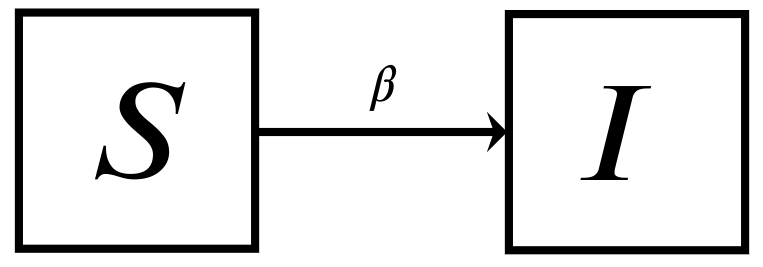
\includegraphics[scale=0.25]{images/img05}
		\caption{Схема перехода индивидов модели SI}
		\label{fig:img05}
	\end{figure}
	
	В первом уравнении дифференциальной задачи \eqref{si-2} расписано количество ушедших из множества здоровых $S(t)$ (левая часть уравнения) как доля заразившихся при контактах (правая часть уравнения). Во втором уравнении количество новоприбывших в множество больных $I(t)$ (левая часть уравнения) расписывается как доля заразившихся при контактах (правая часть уравнения). 
	
	Основным недостатком подхода является предположение о том, что больные и здоровые равномерно распределены по пространству. Как следствие, показатель $\beta$ является константой для всех участников социальной сети, и считается, что контакты происходят между всеми парами <<больной-здоровый>>. Также модель предсказывает на уровне численности и не делает никаких предположений о том, кто именно заболевает в следующий момент времени.
	
	Для дифференциальной задачи \eqref{si-2} мы можем построить как численное, так и аналитическое решение. Причем аналитическое решение данной системы уравнений построить несложно. Для этого, раскрыв скобки, преобразуем систему следующим образом
	$$
		\begin{dcases}
			\dfrac{\d S(t)}{\d t} + \beta\cdot  N \cdot S(t) = \beta \cdot S^2(t),\\
			\dfrac{\d I(t)}{\d t} - \beta\cdot N\cdot I(t) =  -\beta\cdot  I^2(t),\\
			S(0) = S_0,\ I(0) = I_0.
		\end{dcases}
	$$
	Оба уравнения данной системы являются дифференциальными уравнениями Бернулли, для которых можно легко выписать аналитическое решение. В итоге имеем
	\begin{equation}
		S(t) = \dfrac{N \cdot S_0}{-S_0 \cdot e^{\beta \cdot N\cdot t} + S_0 + N\cdot e^{\beta \cdot N \cdot t}},
	\end{equation}
	\begin{equation}
		I(t) = \dfrac{I_0 \cdot N \cdot e^{\beta \cdot N \cdot t}}{I_0\cdot(e^{\beta \cdot N \cdot t} - 1) + N}.
	\end{equation}
	Исследовать методы построения численного решения системы \eqref{si-2} мы не будем. Лишь укажем, что в качестве одного из базовых подходов можно использовать численный метод Рунге-Кутты, который реализован в большинстве пакетов.
	
	Таким образом, SI-модель позволяет нам описывать быстротекущие эпидемии. Если же мы планируем моделировать более серьезные эпидемии, то такая модель будет недостаточно эффективной.
	
	
	\section{Классическая SIR-модель}
	\subsection{Структура модели}
	В популяционных моделях население некоторого региона рассматривается как совокупность групп, как правило, отражающих различный статус индивидов по отношению к заболеванию (восприимчивые, инфицированные, больные в разных стадиях, индивиды в состоянии ремиссии). Внутри каждой группы индивиды считаются неразличимыми между собой. Численности групп меняются со временем в результате следующих процессов:
	\begin{itemize}
		\item переходы индивидов из одной группы в другую вследствие
		инфицирования, развития заболевания, выявления и лечения заболевших
		индивидов;
		\item пополнение групп за счёт иммиграции и рождения индивидов;
		\item убыль в результате естественной смертности индивидуумов, гибели из–за
		болезни и эмиграции в другие регионы.
	\end{itemize}
	Наиболее популярными среди популяционных моделей являются SIR–модели, в которых рассматривается три группы индивидов --- восприимчивые к заболеванию (Susceptible), инфицированные (Infected) и переболевшие либо удалённые
	(Recovered/Removed). Передача инфекции осуществляется от инфицированных
	индивидов к восприимчивым. Переболевшие индивиды приобретают
	иммунитет и не могут быть заражены вторично. Математически такие модели
	задаются системами дифференциальных (непрерывное время) или разностных
	(дискретное время) уравнений. Эти уравнения описывают закон изменения
	численностей групп индивидов с течением времени.
	
	Существуют многочисленные типы моделей, производные от SIR, среди
	которых можно назвать следующие:
	\begin{itemize}
		\item SIRS («Susceptible — Infected — Recovered — Susceptible») – модель,
		описывающая динамику заболеваний c временным иммунитетом
		(выздоровевшие индивиды по прошествии времени опять становятся
		восприимчивыми);
		\item SEIR («Susceptible — Exposed — Infected — Recovered») – модель для
		заболеваний с инкубационным периодом;
		\item SIS («Susceptible — Exposed — Infected) – модель, не учитывающая
		приобретение иммунитета;
		\item MSIR (M — «maternally derived immunity») – модель включает в
		популяцию новорождённых детей, приобретающих иммунитет
		внутриутробно;
		\item и так далее.
	\end{itemize}
	Подробнее вариации этих моделей будут исследованы в п. 1.4.
	\subsection{Достоинства и недостатки}
	Плюсом популяционных SIR–моделей
	является простота в построении и использовании, возможность аналитического
	исследования, лёгкость настройки на реальные данные. Ограничением подхода
	является значительное усложнение математического описания моделей при
	учёте таких факторов, как существенная неоднородность популяции,
	нетривиальная схема передачи инфекции и пр. В детерминированных
	популяционных моделях не может быть учтён фактор случайности в
	распространении заболеваний, особенно значимый в малых популяциях и при
	небольшом числе инфицированных, например, в начальной фазе
	распространения заболевания. Кроме того, в популяционных моделях
	невозможен учёт особенностей отдельных индивидов, что усложняет или
	делает невозможным их использование для решения ряда задач, относящихся к
	эпидемиологии. 
	\subsection{Формулировка SIR-модели в непрерывном времени}
	В качестве примера SIR–модели в непрерывном времени можно привести
	классическую модель Кермака–Маккендрика. Она  основана на разделении населения на три группы: $S$ -- восприимчивые (Susceptible), $I$ -- инфицированные (Infectious) и $R$ -- имеющие иммунитет (Recovered): $$N = S + I + R,$$ где $N$ -- общая численность населения.
	Таким образом, мы можем ввести следующие математические обозначения для переменных и параметров модели. Пусть определено некоторое множество $T \subset \mathbb R$, которое задает некоторый временной промежуток. И пусть также
	\begin{itemize}
		\item $t \in T$ --- независимая переменная, обозначающая некоторый момент времени;
		\item $\beta\in \mathbb R$ -- коэффициент интенсивности контактов индивидов с
		последующим инфицированием;
		\item $\gamma\in \mathbb R$ -- коэффициент интенсивности выздоровления
		инфицированных индивидов;
		\item $S(t): T \to \mathbb R$ -- количество здоровых людей в момент времени $t$; 
		\item $I(t): T \to \mathbb R$ -- количество больных людей в момент времени $t$;
		\item $R(t): T \to \mathbb R$ -- количество переболевших людей в момент времени $t$
		\item $N \in \mathbb R$ --- общая численность населения.
	\end{itemize}
	«Восприимчивые» относятся к группе людей, наиболее уязвимых к заболеванию после контакта с инфицированными людьми. На момент заражения они могут уже быть больными или иметь какое-то хроническое заболевание. Группа «инфицированные» представляет уже зараженных инфекцией людей. Они могут передать болезнь группе восприимчивых людей и могут со временем выздороветь. Выздоровевшие пациенты приобретают иммунитет, так как они больше не подвержены этому заболеванию. [5]
	
	Модель SIR задается в общем виде системой обыкновенных дифференциальных уравнений, на которую накладываются начальные условия. Таким образом, классическая SIR-модель может быть задана в виде задачи Коши
	\begin{equation}
		\begin{dcases}
			\dfrac {\d S(t)}{\d t} = -\beta \cdot S(t) \cdot I(t),\\
			\dfrac{\d I(t)}{\d t} = \beta \cdot S(t)\cdot I(t) - \gamma\cdot I(t),\\
			\dfrac{\d R(t)}{\d t} = \gamma\cdot I(t), \\
			S(0) = S_0,\ I(0) = I_0,\ R(0) = 0.
		\end{dcases}
	\end{equation}
	Это структура, описывающая, как количество людей в каждой группе изменяется в течении времени. 
	
	Схематически эту модель можно представить следующим образом (Рис. 1.2)
	\begin{figure}[h]
		\centering
		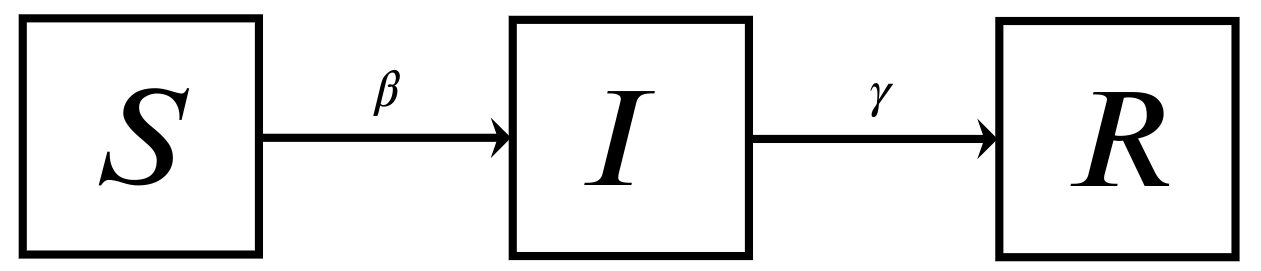
\includegraphics[scale=0.25]{images/img06}
		\caption{Схема перехода индивидов модели SIR}
		\label{fig:img06}
	\end{figure}
	
	\section{Построение задачи Коши для базовой SIR-модели.}
	Рассмотрим начальный момент времени $t_0$, то есть начало эпидемии в данном случае. Пусть у нас имеется один инфицированный индивидуум из группы $I(t)$ и некоторое количество восприимчивых людей из группы $S(t)$. В результате контактов, данный инфицированный индивидуум заражает какое-то количество восприимчивых, тем самым переводит их из группы $S(t)$ в группу $I(t)$, то есть совершается переход $$S \to I.$$
	Введем новую величину $\beta$ -- интенсивность заражения или же  среднее количество контактов на одного человека во времени. Тогда мы можем считать, что один инфицированный заразил в среднем $\beta$ индивидуумов за единицу времени.
	
	Для дальнейшего описания в уравнении (1), предполагая $N\ne 0$, разделим обе части уравнения на $N$ и получим 
	\begin{eqnarray}
		\label{const-eq}
		\dfrac{S(t)}{N} + \dfrac{I(t)}{N} + \dfrac{R(t)}N = 1.
	\end{eqnarray}
	Тогда мы имеем следующие функции:
	\begin{itemize}
		\item $s(t) = \dfrac {S(t)} N$ -- доля подверженных инфицированию индивидуумов;
		\item $i(t) = \dfrac{I(t)} N$ -- доля инфицированных индивидуумов;
		\item $r(t) = \dfrac{R(t)} N$ -- доля выздоровевших, «привитых» и умерших индивидуумов.
	\end{itemize}
	
	Теперь рассмотрим середину эпидемии. Пусть к этому моменту в популяции, кроме двух упомянутых категорий людей, появились переболевшие или выздоровевшие индивидуумы из группы $R(t)$, то есть осуществлялся переход $$I \to R.$$ Рассмотрим конкретного инфицированного и оценим, сколько людей он может заразить. Причем это число уже не равно $\beta$, потому что у нас в популяции есть люди
	невосприимчивые к данной инфекции. Поэтому значение $\beta$ надо уменьшить, а именно умножить на долю всех восприимчивых людей в данный момент времени в популяции $\beta \cdot s(t)$. Таким образом это и есть количество инфицированных людей за единицу времени одним конкретным человеком. 
	
	Общее количество всех инфицированных за единицу времени увеличивается на
	величину $$\beta \cdot s(t) \cdot i(t).$$
	Отметим, что величина $s(t)\cdot i(t)$
	представляет собой плотность контактов между членами групп
	$S(t)$ и $I(t)$.
	
	С другой стороны, изменение величины за единицу времени из физических соображений понимается как скорость, которая определяется как производная этой величины по времени. Тогда мы можем записать введенную  скорость изменения плотности подверженных инфицированию как 
	\begin{eqnarray}
		\label{s-comp}
		\dfrac {\d s(t)}{\d t} = -\beta \cdot s(t) \cdot i(t),
	\end{eqnarray}
	причем доля восприимчивых индивидуумов за единицу времени
	уменьшается на данную величину, поэтому спереди ставим знак « $-$ ».
	Реальное же значение количестве всех инфицированных за единицу времени будет несколько отличаться от наших вычислений, оно будет меньше, так как, разные инфицированные могут заразить одного и того же человека, но мы этим пренебрегаем. 
	
	Далее для исследования изменения доли инфицированных людей за единицу времени мы введем еще одну величину $\gamma$ -- интенсивность выздоровления. Она выражает количество людей, которые
	выздоравливают и переходят в группу $R(t)$ за единицу времени. Например, если болезнь длится $D$ дней, и в течение этого
	периода инфицированный индивидуум может заразить еще кого-то, то $$\gamma = \dfrac 1D.$$
	В среднем $\frac 1D$ всех инфицированных переходит в категорию выздоровевших за единицу времени.
	
	Ввиду определенной величины $\gamma$, мы можем теперь оценить скорость изменения доли инфицированных людей за единицу времени как 
	\begin{eqnarray}
		\label{i-comp}
		\dfrac{\d i(t)}{\d t} = \beta \cdot s(t)\cdot i(t) - \gamma\cdot i(t).
	\end{eqnarray}
	Отметим, что описанная простейшая модель не содержит демографических
	факторов (рождение, смертность от других причин). Таким образом она пригодна для
	краткосрочного прогноза, когда количество новорожденных и умерших за
	рассматриваемый период сравнительно мало (т.е. $N\approx \operatorname{const}$).
	
	Остается определить скорость изменения доли выздоровевших, «привитых» и умерших за единицу времени. С использованием введенных обозначений мы можем ее запросто определить как  
	\begin{eqnarray}
		\label{r-comp}
		\dfrac{\d r(t)}{\d t} = \gamma\cdot i(t).
	\end{eqnarray}
	
	Таким образом, собрав все полученные уравнения \eqref{s-comp}-\eqref{r-comp}, мы получаем систему обыкновенных дифференциальных уравнений
	\begin{equation}
		\label{sir-1}
		\left\{ 
		\begin{gathered} 
			\begin{aligned}
				\dfrac {\d s(t)}{\d t} &= -\beta \cdot s(t) \cdot i(t),\\
				\dfrac{\d i(t)}{\d t} &= \beta \cdot s(t)\cdot i(t) - \gamma\cdot i(t),\\
				\dfrac{\d r(t)}{\d t} &= \gamma\cdot i(t). 
			\end{aligned}
		\end{gathered} 
		\right.		
	\end{equation}
	Причем, сложив все уравнения, мы получим 
	\begin{equation}
		\dfrac {\d s(t)}{\d t} + \dfrac {\d i(t)}{\d t} + \dfrac {\d r(t)}{\d t} = 0,
	\end{equation}
	а в силу уравнения \eqref{const-eq}, имеем 
	\begin{equation}
		\label{const-eq-1}
		s(t) + i(t) + r(t) = 1.
	\end{equation}
	Теперь необходимо поставить задачу для системы уравнений \eqref{sir-1}. Наложим следующие начальные условия 
	\begin{equation}
		\label{constr}
		s(t_0) = s_0 \approx 1,\quad i(t_0) = i_0 << 1,\quad r(t_0) = 0,
	\end{equation}
	которые в нашем случае определяют начало эпидемии следующим образом: в начальный момент времени $t_0$ у нас есть некоторая группа $S(t_0)$ восприимчивых индивидуумов, которая стремится к числу $N$ (так как $s_0 = \frac{S(t_0)}N$), и некоторая группа $I(t_0)$ инфицированных индивидуумов (так как $i_0 = \frac{I(t_0)}N$), которая много меньше $N$, а количество выздоровевших индивидуумов равно нулю.
	
	Собрав воедино систему \eqref{sir-1} и начальные условия \eqref{constr} мы получаем задачу Коши, которая является математической моделью распространения эпидемии 
	$$
	\begin{dcases}
		\dfrac {\d s(t)}{\d t} = -\beta \cdot s(t) \cdot i(t),\\
		\dfrac{\d i(t)}{\d t} = \beta \cdot s(t)\cdot i(t) - \gamma\cdot i(t),\\
		\dfrac{\d r(t)}{\d t} = \gamma\cdot i(t),\\
		s(t_0) = s_0 \approx 1,\quad i(t_0) = i_0 << 1,\quad r(t_0) = 0.
	\end{dcases}
	$$
	\subsection{Корректная постановка задачи Коши для базовой SIR-модели} 
	Рассмотрим систему уравнений SIR-модели:
	\[
	\begin{dcases}
		\dfrac{\mathrm{d}s(t)}{\mathrm{d}t} = -\beta \cdot s(t) \cdot i(t),\\
		\dfrac{\mathrm{d}i(t)}{\mathrm{d}t} = \beta \cdot s(t) \cdot i(t) - \gamma \cdot i(t),\\
		\dfrac{\mathrm{d}r(t)}{\mathrm{d}t} = \gamma \cdot i(t),
	\end{dcases}
	\]
	с начальными условиями:
	\[
	s(t_0) = s_0 \approx 1, \quad i(t_0) = i_0 << 1, \quad r(t_0) = 0.
	\]
	Здесь \( s(t) \), \( i(t) \), \( r(t) \) -- это доли восприимчивого, инфицированного и выздоровевшего населения соответственно. Коэффициенты \( \beta > 0 \) и \( \gamma > 0 \) являются константами (это свойственно SIR-модели), характеризующими скорость передачи инфекции и выздоровления.
	
	Для корректной постановки данной задачи Коши необходимо:
	\begin{itemize}
		\item существование и единственность решения задачи Коши;
		\item устойчивость решения задачи Коши по входным данным.
	\end{itemize}
	
	SIR-модель представляет собой задачу Коши для системы обыкновенных дифференциальных уравнений первого порядка. Согласно теореме о существовании и единственности Пикара–Линдельёфа, решение задачи Коши существует и единственно, если правая часть системы
	\[
	\begin{cases}
		f_1(s, i, r) = -\beta \cdot s(t)\cdot  i(t),\\
		f_2(s, i, r) = \beta \cdot s(t)\cdot  i(t) - \gamma \cdot i(t),\\
		f_3(s, i, r) = \gamma\cdot  i(t),
	\end{cases}
	\]
	удовлетворяет условиям локальной липшицевости. Заметим, что функции \( f_1, f_2, f_3 \) гладкие (дифференцируемы) по всем своим аргументам. Следовательно, система удовлетворяет требованиям теоремы, и для заданных начальных условий \( s_0, i_0, r_0 \) существует единственное решение.
	
	Рассмотрим физический смысл и допустимость решения:
	\begin{enumerate}
		\item Физический смысл переменных:
		\[
		s(t) \geq 0, \quad i(t) \geq 0, \quad r(t) \geq 0, \quad s(t) + i(t) + r(t) = 1.
		\]
		Это следует из интерпретации \( s, i, r \) как долей населения. 
		\item Сохранение суммы \( s(t) + i(t) + r(t) \):
		\[
		\frac{\mathrm{d}}{\mathrm{d}t}(s(t) + i(t) + r(t)) = \frac{\mathrm{d}s}{\mathrm{d}t} + \frac{\mathrm{d}i}{\mathrm{d}t} + \frac{\mathrm{d}r}{\mathrm{d}t} = 0.
		\]
		Таким образом, из начальных условий \( s_0 + i_0 + r_0 = 1 \) следует, что сумма остаётся равной 1 для всех \( t \).
		\item 
		Решение остаётся в области \( s, i, r \geq 0 \), так как:
		\begin{itemize}
			\item Переменная \( s(t) \) убывает (\( \frac{\mathrm{d}s}{\mathrm{d}t} \leq 0 \)).
			\item Переменная \( r(t) \) возрастает (\( \frac{\mathrm{d}r}{\mathrm{d}t} \geq 0 \)).
			\item Переменная \( i(t) \) сначала может расти, но затем убывает.
		\end{itemize}
		Это гарантирует, что решение остается в физически осмысленной области (треугольник $s,i,r \geq 0$, $s+i+r = 1$).
	\end{enumerate}
	
	Начальные условия \( s_0 \approx 1 \), \( i_0 \ll 1 \), \( r_0 = 0 \) соответствуют началу эпидемического процесса, когда почти всё население восприимчиво, а число инфицированных мало. Анализ поведения решения показывает:
	\begin{enumerate}
		\item Если \( \beta s_0 > \gamma \), то \( i(t) \) сначала растёт, что соответствует началу эпидемии.
		\item С течением времени \( i(t) \) убывает, и система стремится к состоянию, где \( i(t) \to 0 \), \( r(t) \to 1 - s(t) \), а \( s(t) \) стабилизируется.
	\end{enumerate}
		
	Таким образом, малые возмущения начальных условий (\( s_0, i_0, r_0 \)) действительно не приводят к разрыву решений или физически бессмысленным значениям.

	Следовательно, задача Коши для SIR-модели является корректно поставленной, и имеет смысл искать ее решение.
	\subsection{Аналитическое решение задачи Коши для базовой SIR-модели}
	Рассмотрим составленную задачу Коши \eqref{sir-1}, \eqref{constr} вместе с уравнением \eqref{const-eq-1}
	$$
	\left\{ 
	\begin{gathered} 
		\begin{aligned}
			\dfrac {\d s(t)}{\d t} &= -\beta \cdot s(t) \cdot i(t),\\
			\dfrac{\d i(t)}{\d t} &= \beta \cdot s(t)\cdot i(t) - \gamma\cdot i(t),\\
			\dfrac{\d r(t)}{\d t} &= \gamma\cdot i(t),
		\end{aligned}
	\end{gathered} 
	\right.
	$$
	$$
	s(t) + i(t) + r(t) = 1,
	$$
	$$
	s(t_0) = s_0,\quad i(t_0) = i_0,\quad r(t_0) = 0,
	$$
	В данной системе дифференциальных уравнений из третьего уравнения выразим $$i(t) = \dfrac1\gamma\cdot \dfrac{\d r(t)}{\d t}$$ и подставим это в первое уравнение:
	$$\dfrac {\d s(t)}{\d t} = -\beta \cdot s(t) \cdot \dfrac1\gamma\cdot\dfrac{\d r(t)}{\d t}.$$
	Перенесем все слагаемые в левую сторону и получим 
	$$\dfrac {\d s(t)}{\d t} +\beta \cdot s(t) \cdot \dfrac1\gamma\cdot\dfrac{\d r(t)}{\d t} = 0.$$
	Получили обыкновенное линейное дифференциальное уравнение относительно неизвестной функции $s(t)$. Домножим обе части уравнения на $$\exp \left(\int\limits_{t_0}^t \dfrac \beta \gamma\cdot \dfrac{\d r(t)}{\d t} \d t \right),$$
	тогда
	$$\dfrac {\d s(t)}{\d t} \exp \left(\int\limits_{t_0}^t \dfrac \beta \gamma\cdot \dfrac{\d r(t)}{\d t} \d t \right) +\beta \cdot s(t) \cdot \dfrac1\gamma\cdot\dfrac{\d r(t)}{\d t} \exp \left(\int\limits_{t_0}^t \dfrac \beta \gamma\cdot \dfrac{\d r(t)}{\d t} \d t \right) = 0.$$
	Полученное выражение слева можно свернуть как производную произведения. Тогда 
	$$\dfrac{\d}{\d t}\left[s(t)\cdot \exp \left(\int\limits_{t_0}^t \dfrac \beta \gamma\cdot \dfrac{\d r(t)}{\d t} \d t \right)\right] = 0.$$
	В итоге мы получили простейшее обыкновенное дифференциальное уравнение первого порядка. Проинтегрируем его с двух сторон по $t$ и получим
	$$s(t)\cdot \exp \left(\int\limits_{t_0}^t \dfrac \beta \gamma\cdot \dfrac{\d r(t)}{\d t} \d t \right) = C,\quad C = \operatorname{const}.$$
	Распишем выражение с $\exp$: $$\exp \left(\dfrac \beta \gamma\cdot\int\limits_{t_0}^t  \dfrac{\d r(t)}{\d t} \d t \right) = \exp \left(\dfrac \beta \gamma\cdot( r(t) - r(t_0))\right) = \exp \left(\dfrac \beta \gamma\cdot r(t)\right).$$
	Тогда, домножив получившееся равенство на $\exp\left(-\frac\beta \gamma r(t)\right)$, получим общее решение уравнения $$s(t) = C \exp\left(-\frac\beta \gamma r(t)\right).$$
	Для определения $C$ подставим начальное условие $s(t_0) = s_0$:
	$$s(t_0) = C = s_0.$$
	Тогда получаем функцию 
	\begin{equation}
		s(t) = s_0 \exp\left(-\frac \beta \gamma r(t)\right).
	\end{equation}
	Теперь, используя уравнение (1.13), выражаем 
	\begin{equation}
		i(t) = 1 - s(t) - r(t) = 1 - s_0 \exp\left(-\frac \beta \gamma r(t)\right) - r(t)
	\end{equation}
	Подставляя это выражение в третье уравнение системы, получаем дифференциальное уравнение 
	\begin{equation}
		\label{drdt-1}
		\dfrac{\d r(t)}{\d t} = \gamma\cdot \big[1 - s_0 \exp\left(-\frac \beta \gamma r(t)\right) - r(t)\big].
	\end{equation}
	Это уравнение является трансцедентным. Трансцендентным уравнением называют уравнение, в котором неизвестная величина является аргументом показательной, логарифмической или тригонометрической функции. Многие уравнения (трансцендентные), не имеют аналитических решений. Однако корни таких уравнений могут быть найдены численными методами с некоторой заранее заданной погрешностью.
	
	В своей работе Кермак и Маккендрик предложили способ отыскания приближенного аналитического решения этого уравнения. В силу предположения, что значение $\frac{\beta}{\gamma} r(t)$ является относительно небольшим, можно приблизить значение $e^{-\frac \beta \gamma r(t)}$ алгебраическим многочленом $$\exp\left(-\frac \beta \gamma r(t)\right) \approx 1 - \frac \beta \gamma r(t) + \dfrac12\left(\dfrac\beta\gamma r(t)\right)^2.$$
	Тогда, подставляя это приближение в выражение \eqref{drdt-1}, имеем обыкновенное дифференциальное уравнение Риккати 
	\begin{equation}
		\label{drdt-2}
		\dfrac{\d r(t)}{\d t} \approx \gamma\cdot \left[1 + \left(\dfrac\beta\gamma s_0 - 1\right)r(t) - \dfrac{s_0\beta ^2}{2 \gamma ^2}r^2(t)\right].
	\end{equation}
	Уравнение \eqref{drdt-2} можно решить как уравнение с разделяющимися переменными, приведя его к виду 
	$$\dfrac{\d r(t)}{\gamma\cdot \left[1 + \left(\dfrac\beta\gamma s_0 - 1\right)r(t) - \dfrac{s_0\beta ^2}{2 \gamma ^2}r^2(t)\right]} \approx \d t.$$
	Проинтегрировав его и выполнив необходимые преобразования, можно получить решение в виде
	\begin{equation}
		r(t)\approx \dfrac{\gamma^2}{\beta^2 s_0}\left[\dfrac{\beta}{\gamma}s_0 - 1 + Q \tanh \left(\dfrac 12Q \gamma t - \tanh^{-1}\dfrac{\frac \beta \gamma s_0 - 1}{Q} \right)\right],
	\end{equation}
	где $$Q = \sqrt{\left(\dfrac \beta \gamma s_0 - 1\right)^2 + 2s_0\dfrac{\beta^2}{\gamma^2}}.$$
	Если ввести замены $$A = \dfrac{\gamma^3 Q^2}{2 s_0 \beta^2},\quad B = \dfrac{Q \gamma }{2},\quad \tanh \varphi = \dfrac{\frac \beta \gamma s_0 - 1}Q,$$
	то можно записать приближенное равенство 
	\begin{equation}
		\dfrac{\d r(t)}{\d t} \approx \dfrac{A}{\cosh^2 (Bt - \varphi)}.
	\end{equation}
	Таким образом, аналитическое решение даже классической SIR-модели строится сильно сложнее, чем для простейшей SI-модели. Также ясно, что точное решение для SIR-модели мы определить не сможем: любое построенное решение задачи Коши будет являться приближенным. Вследствие этого для SIR-моделей и их модификаций решения строятся с помощью численных методов. Поэтому при рассмотрении всех модификаций SIR-модели мы уже не будем останавливаться на построении аналитического решения, а будем ссылаться на возможность построения численного решения.
	\subsection{Приближенное численное решение задачи Коши}
	Ранее мы показали, что задача Коши \eqref{sir-1}, \eqref{constr} является корректно поставленной. А тогда для ее решения мы можем применять численные методы интегрирования обыкновенных дифференциальных систем.
	
	Для того, чтобы построить приближенное численное решение задачи Коши 
	\eqref{sir-1}, \eqref{constr}, можно использовать классические численные методы интегрирования обыкновенных дифференциальных уравнений. К примеру, метод Эйлера, методы Рунге-Кутты, методы предиктор-корректора.
	
	В частности мы будем использовать пакет scipy из Python, в котором предложен алгоритм LSODE (алгоритм Ливермора для обыкновенных дифференциальных уравнений), который решает жесткие и нежесткие системы дифференциальных уравнений первого порядка. В нежестком случае используются методы Адамса (методы предиктор-корректора), а в жестком случае -- методы обратной дифференциации (BDF) (методы Гира). Линейные системы, которые возникают, решаются прямыми методами (LU-факторизация).
	
	Таким образом, вдаваться в формальное представление итерационных алгоритмов численного решения мы не будем. 
	\section{Расширения SIR-модели}
	Все модели, которые мы далее будем рассматривать, основываются на классической SIR-модели, для которой мы описали формальный вывод задачи Коши, обосновали корректную постановку этой задачи Коши и исследовали методы решения этой задачи Коши. Поэтому для всех расширений SIR-модели мы не будем останавливаться на всех этих пунктах, а лишь опишем общую постановку задач Коши при конкретных модификациях классической модели. 
	\subsection{SIS-модель}
	Модель SIS (susceptible-infected-susceptible) основана на предположении, что лица, которые были инфицированы и вылечились, не приобрели
	иммунитет. В этом случае они возвращаются в первую группу восприимчивых $S(t)$. Эта модель описывается следующей задачей Коши:
	\begin{equation}
		\begin{dcases}
			\dfrac{\d S(t)}{\d t} = - \beta\cdot  S(t)\cdot I(t) + \gamma I(t),\\
		\dfrac{\d I(t)}{\d t} = \beta\cdot S(t)\cdot I(t) - \gamma I(t),\\
		S(0) = S_0,\ I(0) = I_0.
		\end{dcases}
	\end{equation}
	В первом уравнении системы описывается переход доли лиц, которые были инфицированы, из группы $S(t)$ в группу $I(t)$. Второе уравнение системы описывает переход
	доли лиц из группы $I(t)$ снова в $S(t)$, т.е. лиц, которые были инфицированы, вылечились и не получили иммунитет. 
	
	Схематически данный процесс представлен на Рис. 1.3
	
	\begin{figure}[h!]
		\centering
		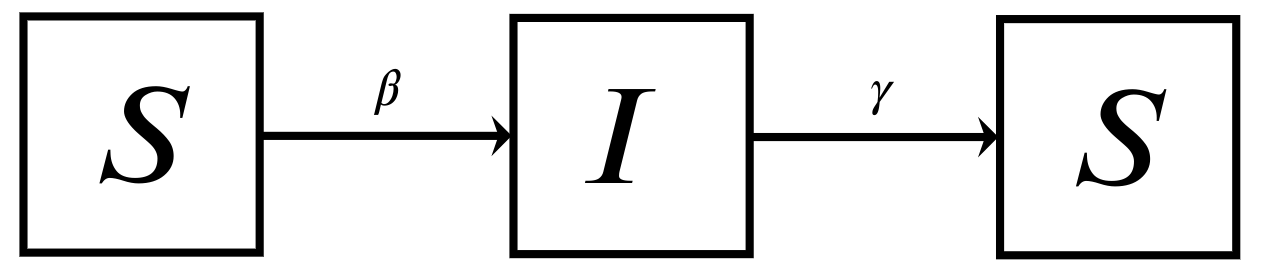
\includegraphics[scale=0.25]{images/img02}
		\caption{Схема перехода индивидов модели SIS.}
		\label{fig:img02}
	\end{figure}
	
	\subsection{SIRD-модель}
	Для описания некоторых инфекционных заболеваний необходимо рассматривать еще одну группу, описывающую долю умерших индивидов. Как правило, эта группа обозначается буквой $D$ (death), а вероятность перехода из группы $I$ в группу $D$ обозначим через $\mu$. Например, к уже описанной модели SIR добавим группу $D$ и получим модель SIRD, которая описывается следующей задачей Коши
	
	\begin{equation}
		\begin{dcases}
			\dfrac {\d S(t)}{\d t} = -\beta \cdot S(t) \cdot I(t),\\
			\dfrac{\d I(t)}{\d t} = \beta \cdot S(t)\cdot I(t) - \gamma\cdot I(t) - \mu\cdot I(t),\\
			\dfrac{\d R(t)}{\d t} = \gamma\cdot I(t), \\
			\dfrac{\d R(t)}{\d t} = \mu\cdot I(t),\\
			S(0) = S_0,\ I(0) = I_0,\ R(0) = 0,\ D(0) = 0.
		\end{dcases}
	\end{equation}
	
	На Рис. 1.4
	приведена схема данной модель. SIRD-модель отличается от классической SIR-модели тем, что инфицированные индивиды могут вылечиться и получить иммунитет с вероятностью $\gamma$ или могут умереть с вероятностью $\mu$. [5]
	\begin{figure}[h]
		\centering
		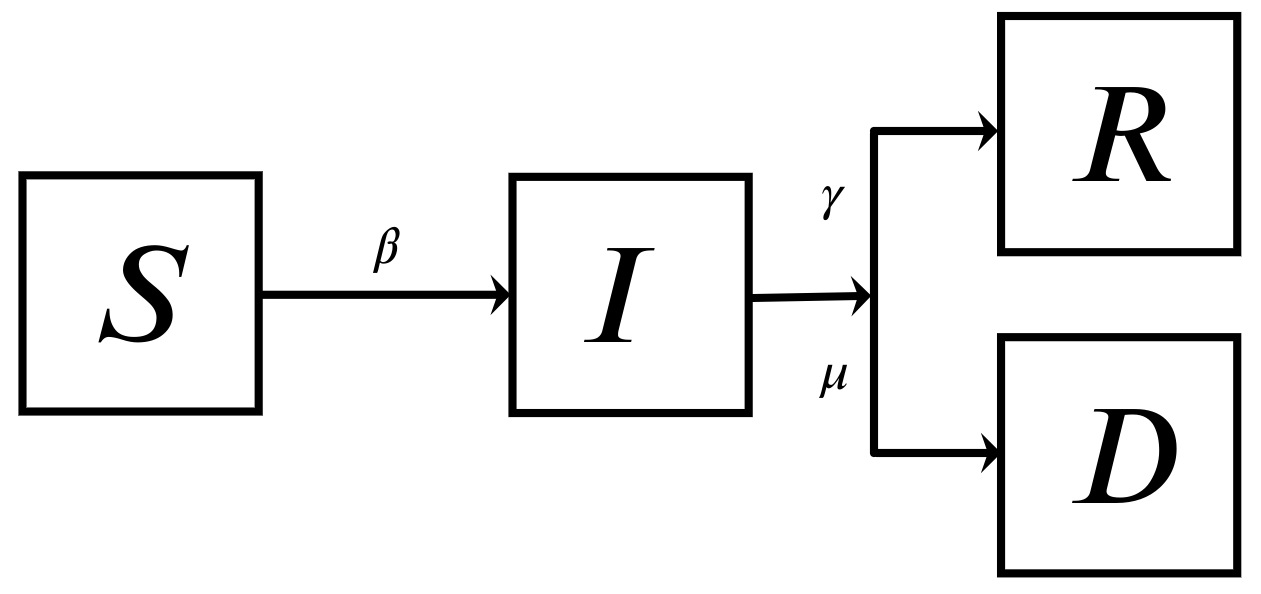
\includegraphics[scale=0.25]{images/img03}
		\caption{Схема перехода индивидов модели SIRD.}
		\label{fig:img03}
	\end{figure}
	
	\subsection{SIRS-модель}
	Модель SIRS (Susceptible-Infected-Recovered-Susceptible) является вариацией модели SIR, которая учитывает возможность повторного заражения после выздоровления (потери иммунитета). В модели SIRS существует циклическое движение между группами подверженных $S$, инфицированных $I$ и восстановленных $R$. Эта модель описывается задачей Коши
	\begin{equation}
	\begin{dcases}
		\dfrac {\d S(t)}{\d t} = -\beta \cdot S(t) \cdot I(t) + \lambda \cdot R(t),\\
		\dfrac{\d I(t)}{\d t} = \beta \cdot S(t)\cdot I(t) - \gamma\cdot I(t),\\
		\dfrac{\d R(t)}{\d t} = \gamma\cdot I(t) - \lambda \cdot R(t),\\
		S(0) = S_0,\ I(0) = I_0,\ R(0) = 0.
	\end{dcases}
	\end{equation}
	где число $\lambda$ определяет вероятность потери иммунитета и перехода из группы $R(t)$ в группу $I(t)$. [2]
	
	Схематически эту модель можно представить следующим образом (Рис. 1.5)
	\begin{figure}[h]
		\centering
		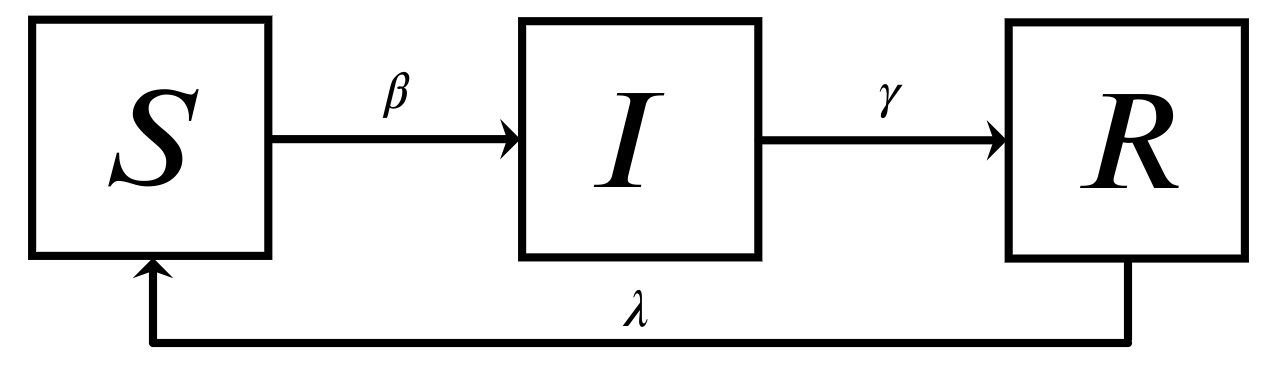
\includegraphics[scale=0.25]{images/img07}
		\caption{Схема перехода индивидов модели SIRS}
		\label{fig:img07}
	\end{figure}
	
	Модель SIRS позволяет изучать повторные вспышки болезни в популяции, так как люди, выздоровевшие от инфекции, могут снова стать подверженными и инфицироваться. Это особенно важно для изучения болезней, которые не обеспечивают долгосрочный иммунитет, например, грипп или коронавирусные инфекции.
	
	\subsection{Модели с учетом смертности и рождаемости особей}
	Для моделирования процессов распространения инфекционных заболеваний в длительные периоды времени необходимо учитывать процессы рождаемости и смертности.
	
	Пусть $\lambda = \operatorname{const} > 0$ и $\mu = \operatorname{const} > 0$ -- это коэффициенты рождаемости и смертности популяции соответственно. Задача Коши для описания SIR-модели в предположении, что все рожденные являются здоровыми людьми, имеет вид 
	\begin{equation}
		\begin{dcases}
		\dfrac {\d S(t)}{\d t} = -\beta \cdot S(t) \cdot I(t) + \lambda\cdot N(t) - \mu\cdot S(t),\\
		\dfrac{\d I(t)}{\d t} = \beta \cdot S(t)\cdot I(t) - \gamma\cdot I(t) - \mu\cdot I(t),\\
		\dfrac{\d R(t)}{\d t} = \gamma\cdot I(t) - \mu \cdot R(t),\\
		S(0) = S_0, \ I(0) = I_0,\ R(0) = 0.
		\end{dcases}
	\end{equation}
	где $$S(t) + I(t) + R(t) = N(t),$$ причем заметим, что теперь численность популяции -- это функция $N = N(t)$, то есть она непостоянная (за счет рождаемости и смертности людей). [5]
	
	Складывая все уравнения системы, мы получаем уравнение Мальтуса для численности популяции 
	\begin{equation}
	\dfrac{\d N(t)}{\d t} = (\lambda-\mu) \cdot N(t).
	\end{equation}
	
	Анализируя поведение $I'(0)$, можно определить базовое репродуктивное число. Для отсутствия эпидемии необходимо, чтобы $$\beta S_0 - \gamma - \mu < 0 \quad \text{или}\quad \beta \dfrac{S_0}{\Lambda+\mu} < 1.$$
	Следовательно имеем базовое репродуктивное число для расширенной модели $$R_0 = \beta \cdot \dfrac{S_0}{\Lambda+\mu}.$$ Обратим внимание на то, что коэффициент рождаемости не влияет на пороговый
	эффект. Расширенная SIR-модель с учетом рождаемости и смертности может иметь колеблющиеся решения.
	
	\subsection{SEIR-модель, или модель с учетом инкубационного периода}
 	Очень часто стандартная модель SIR является слишком простой и
	нереалистичной, так как в ней полагается, что особь является заразной сразу же после инфицирования. В SEIR модели предполагается, что инфекция имеет инкубационный период, в течение которого люди инфицированы, но
	еще не заразны. Эта группа людей обозначается через $E$ (exposed). С учетом нового класса получаем следующую структуру
	популяции:
	$$S + E + I + R = N,$$ где
	\begin{itemize}
		\item $S(t)$ -- это количество не инфицированных людей. Причем скорость изменения количества подверженных зависит от вероятности передачи инфекции, количества инфицированных и количества подверженных, где $\beta$ -- это скорость передачи заболевания;
		\item $E(t)$ -- это число инфицированных, но еще не заразных людей. Причем скорость изменения количества инфицированных, но еще не заразных людей зависит от входящего потока людей, проходящих инкубационный период, а также выходящего потока этих же людей. Параметр $\sigma^{-1}$ представляет собой среднюю продолжительность инкубационного периода;
		\item $I(t)$ -- это количество инфицированных людей. Причем	скорость изменения количества инфицированных зависит от входящего потока инфицированных и выходящего потока инфицированных. Параметр $\gamma$ -- это скорость восстановления;
		\item $R(t)$ -- это группа выздоровевших лиц, а именно людей, которые восстановились.
	\end{itemize}
	Модель SEIR описывается задачей Коши
	\begin{equation}
		\begin{dcases}
		\dfrac {\d S(t)}{\d t} = - \beta \cdot I(t)\cdot S(t),\\
		\dfrac {\d E(t)}{\d t} = \beta \cdot S(t)\cdot I(t) - \sigma\cdot E(t),\\
		\dfrac{\d I(t)}{\d t} =\sigma \cdot E(t) - \gamma\cdot I(t),\\
		\dfrac{\d R(t)}{\d t} = \gamma\cdot I(t),\\
		S(0) = S_0,\ I(0) = I_0,\ E(0) = 0,\ R(0) = 0.
		\end{dcases}
	\end{equation}
	
	Схематически эта модель может быть записана в следующем виде (Рис. 1.6)
	\begin{figure}[h]
		\centering
		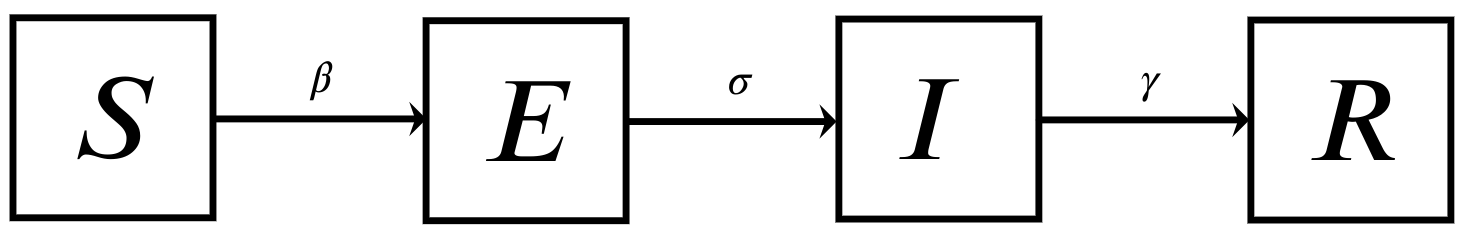
\includegraphics[scale=0.3]{images/img08}
		\caption{Схема перехода индивидов модели SEIR}
		\label{fig:img08}
	\end{figure}
	
	
	Также имеет место модель SEIR с учетом смертности и рождаемости особей, которая описывается задачей Коши
	\begin{equation}
	\begin{dcases}
		\dfrac {\d S(t)}{\d t} = \lambda N(t) - (\beta \cdot I(t) +\mu)\cdot S(t),\\
	\dfrac {\d E(t)}{\d t} = \beta \cdot S(t)\cdot I(t) - (\mu + \sigma)\cdot E(t),\\
	\dfrac{\d I(t)}{\d t} =\sigma \cdot E(t) - (\mu + \gamma)\cdot I(t),\\
	\dfrac{\d R(t)}{\d t} = \gamma\cdot I(t) - \mu \cdot R(t),\\
	S(0) = S_0,\ I(0) = I_0,\ E(0) = 0,\ R(0) = 0.
	\end{dcases}
	\end{equation}
	
	
	Важно отметить, что модель SEIR является упрощенной моделью и не учитывает множество реальных факторов, таких как вакцинация, мутации вируса и изменение поведения людей. Но она предоставляет базовый фреймворк для изучения распространения инфекции и позволяет прогнозировать общую динамику эпидемии.
	Именно на примере этой модели мы и будем проводить эксперименты в главе 3.
	
	Дополнительные вариации модели SEIR также могут включать дополнительные факторы, такие как иммунизация или введение противоэпидемических мер. Модель SEIR и ее вариации широко используются в исследованиях эпидемиологии и планировании общественного здравоохранения. Они позволяют ученым и решающим органам оценить различные стратегии контроля эпидемии, такие как вакцинация, социальное дистанцирование, использование масок и карантинные меры. Такие модели могут помочь прогнозировать будущие тенденции распространения болезни и определить наиболее эффективные меры по сдерживанию инфекции.
	
	\subsection{MSIR-модель}
	Модель MSIR (M — «maternally derived immunity») включает класс $M(t)$ (для материнского иммунитета) в начало модели. При многих инфекциях, включая корь, младенцы рождаются невосприимчивыми к этому заболеванию, но в течение первых нескольких месяцев жизни обладают иммунитетом к этому заболеванию благодаря защите от материнских антител (которые передаются через плаценту и дополнительно через молозиво). Это называется пассивным иммунитетом. Эту дополнительную деталь можно продемонстрировать, включив в начало модели класс $M(t)$ (для иммунитета, передающегося по материнской линии). 
	
	Модель MSIR мы будем строить на основе модели с учетом смертности и рождаемости. Тогда модель MSIR описывается следующей задачей Коши
	\begin{equation}
	\begin{dcases}
	\dfrac {\d M(t)}{\d t} = \lambda \cdot N(t) - \delta\cdot M(t)-\mu\cdot M(t),\\
	\dfrac {\d S(t)}{\d t} = \delta \cdot M(t) -\beta\cdot S(t)\cdot I(t) - \mu \cdot S(t),\\
	\dfrac{\d I(t)}{\d t} =\beta\cdot S(t)\cdot I(t) - \gamma \cdot I(t) - \mu \cdot I(t),\\
	\dfrac{\d R(t)}{\d t} = \gamma\cdot I(t) - \mu \cdot R(t),\\
	M(0) = M_0,\ S(0) = S_0,\ I(0) = I_0,\ R(0) = 0.
	\end{dcases}
	\end{equation}
	где, $\delta$ -- это вероятность потери материнского иммунитета, $\lambda$ и $\mu$ -- это коэффициенты рождаемости и смертности популяции соответственно и $$S(t) + I(t) + R(t) = N(t).$$
	
	Схематически эта модель может быть записана в следующем виде (Рис. 1.7)
	\begin{figure}[h]
		\centering
		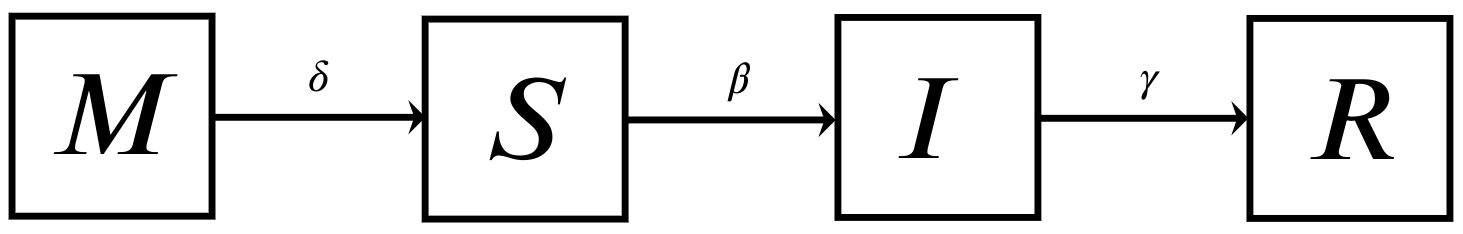
\includegraphics[scale=0.3]{images/img09}
		\caption{Схема перехода индивидов модели MSIR}
		\label{fig:img09}
	\end{figure}
	
	\subsection{MSEIR-модель}
	Теперь усложним модель SEIR с учетом смертности и рождаемости особей, добавив к ней материнский иммунитет. Таким образом, получается модель MSEIR.
	Модель MSEIR ($M$ -- наделенные иммунитетом от рождения, $S$ -- восприимчивые, $E$ -- контактные, $I$ -- инфицированные, $R$ -- выздоровевшие) -- одна из самых сложных для анализа в силу наличия большого числа независимых параметров. Задача Коши для нее имеет вид
	\begin{equation}
		\begin{dcases}
		\dfrac {\d M(t)}{\d t} = \lambda \cdot N(t) - \delta\cdot M(t)-\mu\cdot M(t),\\
		\dfrac {\d S(t)}{\d t} = \delta \cdot M(t) -\beta\cdot S(t)\cdot I(t) - \mu \cdot S(t),\\
		\dfrac {\d E(t)}{\d t} = \beta \cdot S(t)\cdot I(t) - (\sigma + \mu)\cdot E(t),\\
		\dfrac{\d I(t)}{\d t} =\sigma \cdot E(t) - (\gamma + \mu)\cdot I(t),\\
		\dfrac{\d R(t)}{\d t} = \gamma\cdot I(t) - \mu \cdot R(t),\\
		M(0) = M_0,\ S(0) = S_0,\ I(0) = I_0,\ E(0) = 0,\ R(0) = 0.
		\end{dcases}
	\end{equation}
	где $M (t)$ -- численность индивидов с приобретенным внутриутробно иммунитетом. От ранее рассмотренных моделей эта система отличается тем, что учитывает рождение детей, вероятность заражения которых растет со временем по мере утраты ими иммунитета, приобретенного внутриутробно. Эти зависимости описаны в первых двух уравнениях системы. [5]
	
	Схематически эта модель может быть записана следующим образом (Рис. 1.8)
	\begin{figure}[h!]
		\centering
		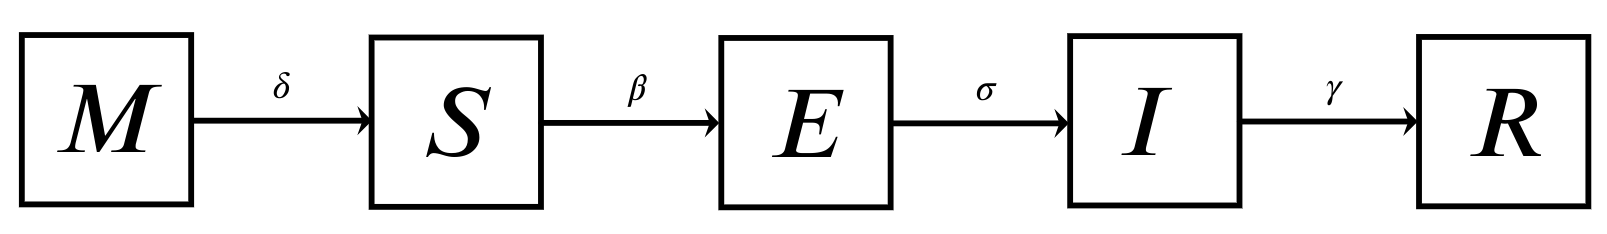
\includegraphics[scale=0.3]{images/img10}
		\caption{Схема перехода индивидов модели MSEIR}
		\label{fig:img10}
	\end{figure}
	
	Таким образом, в зависимости от условия протекания эпидемии мы можем модифицировать базовую SIR-модель, добавляя к ней новые группы или изменяя условия переходов из одной группы в другую. Эта универсальность позволяет учитывать множество факторов, влияющих на распространение болезни. Однако стоит также учитывать, что, добавляя новые факторы и группы, модель становится сильно сложнее. Это можно было наблюдать при сравнении SI и SIR моделей, когда, добавив одну новую группу, мы утратили возможность строить аналитическое решение дифференциальной системы.
	
	
	\newpage
	\chapter{РАСШИРЕННЫЕ МЕТОДЫ МОДЕЛИРОВАНИЯ ЗАБОЛЕВАНИЙ НА ОСНОВЕ БАЗОВЫХ МОДЕЛЕЙ}
	Для конкретики все дальнейшие расширенные методы моделирования заболеваний мы будем рассматривать, взяв в качестве базовой модели SEIR-модель, так как в главе 3 мы будем проводить практические эксперименты основываясь именно на данной модели. 
	
	Классическая SEIR-модель описывается задачей Коши
	Модель SEIR описывается задачей Коши
	\begin{equation*}
		\begin{dcases}
			\dfrac {\d S(t)}{\d t} = - \beta \cdot I(t)\cdot S(t),\\
			\dfrac {\d E(t)}{\d t} = \beta \cdot S(t)\cdot I(t) - \sigma\cdot E(t),\\
			\dfrac{\d I(t)}{\d t} =\sigma \cdot E(t) - \gamma\cdot I(t),\\
			\dfrac{\d R(t)}{\d t} = \gamma\cdot I(t),\\
			S(0) = S_0,\ I(0) = I_0,\ E(0) = 0,\ R(0) = 0.
		\end{dcases}
	\end{equation*}
	
	В контексте данной главы эту SEIR-модель мы будем называть \textit{детерминированной}.
	\section{Вероятностные популяционные модели}
	Общая идея построения стохастических популяционных SIR-моделей и их обобщений аналогична их детерминированным аналогам:
	популяция рассматривается как совокупность групп, внутри каждой из которых
	индивиды считаются неразличимыми между собой. Различие проявляется в
	описании законов перехода индивидов между группами. В качестве
	математического аппарата применяются системы стохастических разностных
	уравнений, цепи Маркова, случайные процессы в дискретном и непрерывном
	времени (процессы Гальтона–Ватсона, процессы рождения и гибели и пр.). 
	
	В отличие от детерминированных SIR-моделей, в стохастических имитационных моделях корректно учитывается
	фактор случайности. В то же время стохастические популяционные модели
	сложнее для аналитического исследования по сравнению с аналогичными
	детерминированными. Полноценное аналитическое исследование возможно
	лишь для некоторых простых типов моделей, в общем же случае для оценки
	динамики численностей групп обычно прибегают к имитационному
	моделированию с помощью методов Монте–Карло. Имитационные модели на
	базе SIR–моделей обладают высокой производительностью, в результате чего
	они до сих пор широко применяются в программных комплексах.
	
	Вместо детерминистского подхода, где изменения в группах $S, E, I, R$ описываются системой дифференциальных уравнений, мы переходим к вероятностной модели. Здесь мы моделируем случайные события (например, заражение, выздоровление) как процессы, происходящие с заданными вероятностями. Причем ввиду того, что случайные величины могут быть как дискретными, так и непрерывными, то у нас имеются два варианта построения вероятностных моделей: с дискретным временем и с непрерывным временем.
	
	\subsection{Вероятностная модель с дискретным временем}
	В дискретной модели состояние популяции обновляется через конечные шаги времени 
	$t=0,1,2,\ldots$. Пусть $S_t, E_t, I_t, R_t$
	обозначают числа восприимчивых, экспонированных, инфекционных и выздоровевших индивидов соответственно на временном шаге $t$. Общая популяция в таком случае остается постоянной:
	$$N = S_t + E_t + I_t + R_t.$$
	
	Основная цель вероятностного подхода заключается в том, чтобы сделать переходы из одной группы в другую, которые на данный момент зависят лишь от чисел $\beta, \sigma,\gamma$, случайными. То есть для описания перехода из одной группы в другую мы должны использовать аппарат случайных величин.
	
	Итак, пусть $\Delta t$ обозначает один шаг по времени (например, это может быть 1 день). Тогда мы можем определить следующие случайные величины
	\begin{enumerate}
		\item Переход $S \to E$. Вероятность того, что восприимчивый человек $S$ заразится за один временной шаг $\Delta t$, определяется как
		$$
		P_{S\to E} = 1 - \exp\left(-\beta\cdot  \frac{I}{N} \cdot \Delta t\right)
		$$
		где $\beta$ -- коэффициент передачи инфекции, $\frac{I}{N}$ -- вероятность контакта с зараженным. Тогда число восприимчивых людей, инфицированных за промежуток времени $\Delta t$ описывается случайной величиной
		$$\Delta E_t \sim \Binom(S_t, P_{S\to E}).$$
		\item Переход $E \to I$. Зараженные, но не заразные люди $E$ становятся заразными $I$ за один временной шаг $\Delta$ с вероятностью
		$$
		P_{E\to I} = 1 - \exp\left(-\sigma \cdot \Delta t\right)
		$$
		где $\sigma = \frac{1}{T_E}$ -- обратная продолжительность инкубационного периода. Тогда число людей, перешедших в активную фазу заболевания за промежуток времени
		$\Delta t$ описывается случайной величиной
		$$\Delta I_t \sim \Binom(E_t, P_{E\to I}).$$
		\item Переход $I \to R$. Инфицированные $I$ выздоравливают и переходят в группу $R$ за временной шаг $\Delta t$ с вероятностью
		$$
		P_{I\to R} = 1 - \exp\left(-\gamma \cdot \Delta t\right)
		$$
		где $\gamma$ -- это коэффициент восстановления. Тогда число людей, удаленных из популяции (вследствие выздоровления
		или гибели)
		$\Delta t$ описывается случайной величиной
		$$\Delta R_t \sim \Binom(I_t, P_{I\to R}).$$
	\end{enumerate}
	Тогда из исходной задачи Коши для описания детерминированной SEIR-модели мы получаем разностную задачу для описания стохастической SEIR-модели с дискретным временем
	\begin{equation}
		\begin{dcases}
			S_{t+1} = S_t - \Delta E_t,\\
			E_{t+1} = E_t +\Delta E_t - \Delta I_t,\\
			I_{t+1} = I_t + \Delta I_t - \Delta R_t,\\
			R_{t+1} = R_t + \Delta R_t,
		\end{dcases}
		t = 0,1,2\ldots,
	\end{equation}
	где $S_0$ и $I_0$ заданы, а $E_0 = R_0 = 0$.
	
	Очевидно, что каждая реализация данной разностной задачи будет давать различный результат, поскольку в ней фигурируют случайные величины. 
	\subsection{Вероятностная модель с непрерывным временем}
	В непрерывной версии модели состояние популяции описывается с помощью стохастического процесса, часто представляемого как цепь Маркова или процесс Пуассона.
	
	Пусть $S(t), E(t), I(t), R(t)$ -- это состояния системы в момент времени $t$. Общая популяция остается постоянной
	$$N = S(t) + E(t) + I(t) + R(t).$$
	
	Зададим непрерывную модель как процесс Пуассона, задаваемый интенсивностями переходов:
	\begin{enumerate}
		\item Заражение $S \to E$:
		$$\lambda_{SE} = \dfrac{\beta \cdot S(t) \cdot I(t)}{N}.$$
		\item Переход в инфекционное состояние $E \to I$:
		$$\lambda_{EI} = \sigma \cdot E(t).$$
		\item Выздоровление $I \to R$:
		$$\lambda _{IR} = \gamma \cdot I(t).$$
	\end{enumerate}
	
	С учетом введенных интенсивностей изменения численности групп за малый интервал $\Delta t$ задаются как случайные величины из распределения Пуассона
	$$\Delta E \sim \Pois(\lambda_{SE} \cdot \Delta t),$$
	$$\Delta I \sim \Pois(\lambda_{EI} \cdot \Delta t),$$
	$$\Delta R \sim \Pois(\lambda_{IR} \cdot \Delta t).$$
	
	В итоге, исходя из детерминированной задачи Коши, можем описать стохастическую SEIR-модель с непрерывным временем как
	\begin{equation}
		\begin{cases}
			S(t+\Delta t) = S(t) - \Delta E,\\
			E(t+\Delta t) = E(t) + \Delta E - \Delta I,\\
			I(t + \Delta t) = I(t) + \Delta I - \Delta R,\\
			R(t + \Delta t) = R(t) + \Delta R.
		\end{cases}
	\end{equation}
	\newpage
	\subsection{Сравнение вероятностных моделей с дискретным и непрерывным временем}
	Сравним основные характеристики обеих рассмотренных моделей
	\begin{table}[h]
		\renewcommand{\arraystretch}{1}
		\begin{tabular}{|p{4cm}|p{5.5cm}|p{5.5cm}|}
			\hline
			\textbf{Характеристика} & \textbf{Дискретное время} & \textbf{Непрерывное время} \\ \hline
			Обновление состояния & Состояние обновляется на каждом шаге \( t \) & Состояние меняется как процесс Пуассона \\ \hline
			События & Моделируются биномиальными распределениями & Моделируются пуассоновскими процессами \\ \hline
			Применение & Удобна для численного моделирования & Более точна для моделирования реального времени \\ \hline
			Интенсивности переходов & Вероятности событий за шаг времени & Скорости событий (интенсивности) \\ \hline
		\end{tabular}
		\caption{Сравнение дискретной и непрерывной SEIR-моделей}
	\end{table}
	\subsection{Реализация вероятностных моделей}
	Программно реализовать вероятностные модели можно с помощью численных алгоритмов. Однако каждая реализация численного алгоритма будет отличаться от остальных, поскольку на каждом шаге мы генерируем случайную величину. Вследствие этого для таких моделей принято рассчитывать $K=1,2,\ldots$ реализаций, а в качестве результата брать усредненные значения с учетом доверительного интервала. 
	Для каждой модели и каждой из групп $S, E, I, R$ можно рассчитать доверительные интервалы, используя:
	$$
	CI = \bar{X} \pm z \cdot \frac{\sigma}{\sqrt{n}}
	$$
	где $\bar{X}$ -- среднее значение, $\sigma$ -- стандартное отклонение, $z$ -- квантиль нормального распределения (например, $z = 1.96$ для 95\% доверительного интервала).
	
	Таким образом, детерминированная модель дает гладкое среднее значение, не учитывая случайные колебания, а динамическая стохастическая модель позволяет учитывать случайные колебания (например, шум), что делает ее более реалистичной.
	
	\section{Имитационные модели с пространственной структурой}
	В ряде задач математической эпидемиологии
	возникает необходимость учёта географической и социальной неоднородности
	популяции, которая не может быть описана популяционными моделями. В этом
	случае применяются имитационные модели, включающие в себя
	пространственные структуры. В зависимости от типа доступных
	пространственных данных и решаемого класса задач, могут быть использованы
	метапопуляционные модели, клеточные автоматы, сетевые модели либо модели
	с привлечением географических информационных систем. В первых трёх
	случаях в модели может рассматриваться не пространственная близость
	индивидов популяции, а их близость в социальном отношении (социальные
	связи).
	
	\subsection{Клеточные автоматы}
	
	Первые имитационные модели в качестве пространственной структуры
	использовали \textit{клеточные автоматы}. В простейшем случае клеточный автомат —
	это прямоугольная двумерная решетка, каждый узел которой в фиксированный
	момент времени находится в одном из конечного числа состояний (к примеру,
	для SIR–модели узел представляет собой индивида в состоянии
	«восприимчивый», «инфицированный» или «переболевший»). Как правило,
	индивиды полностью отождествляются с узлом, который они занимают. В
	случае, если индивиды перемещаются по сетке, полученную модель правильнее
	относить к более общему классу — классу сетевых моделей, о котором речь
	пойдкт далее.
	
	В клеточном автомате принимается некоторая схема соседства, согласно
	которой определяются узлы, смежные с данным — его «соседи» — четыре
	соседа, восемь соседей или, при более сложных схемах соседства,
	произвольное число. Иногда для имитации «дальних» контактов (к примеру,
	случайных встреч незнакомых людей в общественных местах) считается, что в
	каждый фиксированный момент времени помимо узлов, смежных с данным в
	пространственной решетке, соседями рассматриваемого узла являются
	несколько произвольно выбранных во всей решетке узлов.
	
	Время в клеточных автоматах дискретное, на каждом шаге все состояния
	узлов решетки меняются в соответствии с выбранным правилом перехода,
	являющимся функцией от состояний соседей фиксированного узла. Если
	правило перехода детерминированное (например, если больше половины
	соседей индивида инфицированы, то он тоже становится инфицированным), то
	клеточный автомат называется детерминированным. Если же это правило
	имеет вероятностный характер (например, индивид, имеющий хотя бы одного инфицированного соседа, становится инфицированным с вероятностью p), то
	автомат называется вероятностным (стохастическим).
	
	Поскольку подход с использованием клеточных автоматов является
	достаточно общим, соответствующие имитационные модели могут
	применяться для решения большого круга задач математической
	эпидемиологии. 
	
	\subsection{Сетевые модели}
	
	Более гибким способом моделирования пространственной неоднородности
	является использование сетей. Аналогично клеточным автоматам, в
	\textit{классических сетевых моделях} распространения инфекций индивиды
	обозначаются узлами, при этом каждый индивид может иметь произвольное
	количество связей с другими индивидами (социальных либо пространственных).
	Эти связи обозначаются дугами. Различают статические сети, в которых
	количество узлов и связи между ними неизменны, и динамические, в которых
	они могут меняться с некоторым шагом по времени. Если узлы сети, помимо
	состояния, связанного с заболеваемостью («восприимчивый»,
	«инфицированный» или «переболевший»), имеют набор параметров, то сетевая
	модель становится индивидуум–ориентированной.
	
	Одним из главных плюсов простых
	имитационных пространственных моделей является возможность их
	использования для построения простых моделей пространственно
	неоднородных популяций, не требующих большого количества входных
	данных. Минусом является недостаточная реалистичность моделирования
	пространственных отношений из–за применения регулярной пространственной
	структуры.
	
	Достоинством сетевых моделей является их гибкость, позволяющая
	наиболее полно отражать все аспекты распространения заболеваний, связанные
	с пространственной неоднородностью популяции. В частности, в отличие от
	клеточных автоматов, они позволяют моделировать такие важные явления, как
	кластеризацию популяции (наличие групп с высокой связностью узлов друг с
	другом), «суперраспространителей» (индивидов, имеющих наибольшее
	количество связей, заражение которых влечёт быстрое распространение
	инфекции) и пр. В связи с этим с помощью сетевых моделей возможно
	изучение некоторых нетривиальных режимов распространения эпидемий, не
	воспроизводимых популяционными моделями и клеточными автоматами.
	Минусом является повышение сложности модели, что требует дополнительных
	данных для проведения вычислительных экспериментов.
	\subsection{Постановка задачи для пространственной модели}
	Рассмотрим вероятностную модель распространения инфекции, но добавим учет пространственной неоднородности. Пространственная неоднородность важна, так как инфекция распространяется неравномерно: люди имеют ограниченные социальные контакты, живут в разных регионах и перемещаются. Мы рассмотрим модель на основе клеточных автоматов, чтобы учесть пространственную структуру популяции.
	
	Клеточные автоматы -- это удобный инструмент для моделирования пространственных процессов, таких как распространение инфекции. В такой модели
	
	\begin{itemize}
		\item пространство делится на дискретные ячейки (регион, квартал, город и т.д.);
		\item каждая ячейка имеет состояние (например, $S$, $E$, $I$, $R$);
		\item состояние каждой ячейки обновляется во времени в зависимости от её текущего состояния и состояния соседей.
	\end{itemize}
	
	Клеточные автоматы хорошо подходят для моделирования локальных взаимодействий и пространственного распространения инфекции.
	
	Пусть пространство задается как двумерная сетка размера $M\times N$, где каждая ячейка представляет некоторую область (например, это может быть город или район).
	Каждая из ячеек имеет одно из состояний:
	\begin{itemize}
		\item $S$ -- восприимчивые;
		\item $E$ -- инфицированные в инкубационном периоде;
		\item $I$ -- заразные;
		\item $R$ -- выздоровевшие.
	\end{itemize}
	В каждой ячейке инфекция распространяется с некоторой вероятностью, зависящей от
	\begin{itemize}
		\item численности зараженных в текущей ячейке;
		\item численности зараженных в соседних ячейках.
	\end{itemize}
	Опишем механику всего процесса.
	Восприимчивые $S$ могут заразиться от инфицированных $I$ в той же ячейке или в соседних ячейках. Вероятность заражения зависит от коэффициента передачи $\beta$ и числа зараженных.
	Как и в модели SEIR, индивиды переходят между состояниями $E, I, R$ с вероятностями, зависящими от параметров $\sigma$ (инкубационный период) и $\gamma$ (выздоровление).
	Однако в отличие от детерминированной SEIR-модели, соседние ячейки могут влиять друг на друга. Например, если в одной ячейке много зараженных, соседние ячейки получают дополнительный риск заражения.
	\subsection{Реализация пространственной модели}
	Опишем алгоритм реализации пространственной модели.
	Сперва, исходя из постановки пространственной задачи, необходимо создать двумерную сетку $M\times N$, где каждая ячейка содержит численности $S,E,I,R$. Далее на каждом временном шаге:
	\begin{itemize}
		\item для каждой ячейки рассчитывается вероятность заражения с учетом соседей;
		\item обновляются состояния ячеек (заражение, выздоровление, переходы между состояниями).
	\end{itemize}
	Для остановки цикла необходимо задать верхнюю границу для времени, то есть период времени, в течение которого моделируется эпидемия.
	\section{Индивидуум-ориентированные и мультиагентные методы моделирования}
	В рамках индивидуум-ориентированного подхода каждый
	индивид наделяется набором параметров, описывающих его внутренние
	особенности, пространственное расположение, социальный статус и показатели,
	связанные с протеканием заболевания. Часто индивидуум–ориентированные
	модели строятся на основе пространственных структур, но в общем случае они
	могут и отсутствовать.
	
	Среди индивидуум-ориентированных моделей выделяется подкласс,
	включающий в себя так называемые мультиагентные модели. Принадлежность
	индивидуум–ориентированной модели к классу мультиагентных, как правило,
	определяется тем, что индивиды в них моделируются как независимые сущности с определённым шаблоном поведения. В результате действий
	отдельных агентов, направленных на достижение индивидуальных целей, у
	системы наблюдаются некоторые свойства, не присущие её отдельным
	элементам.
	
	Следует отметить, что в ряде работ модели называются «индивидуум–
	ориентированными» или даже «мультиагентными» в случае, если в моделях
	происходит обращение к индивидам как к отдельным сущностям (в отличие от
	классических популяционных моделей, которые манипулируют численностями
	групп индивидов), при этом сами индивиды могут быть не отличимыми друг от
	друга.
	
	Бесспорным достоинством индивидуум-ориентированного подхода является возможность сколь угодно детального
	описания свойств индивидов, влияющих на распространение болезни в
	популяции. Благодаря этому индивидуум-ориентированные модели позволяют
	задавать процессы в неоднородных популяциях с наиболее высокой степенью
	достоверности. Вместе с тем, многопараметрическое описание индивидов
	приводит к необходимости в детальных данных для калибровки моделей и
	значительных вычислительных ресурсах для проведения экспериментов. Кроме
	того, переусложненные модели неудобны в обращении и результаты их работы
	сложно интерпретировать. По этим причинам важно найти удачный
	компромисс между реалистичностью разрабатываемых моделей и их
	наглядностью.
	
	\subsection{Постановка задачи для мультиагентной модели}
	В модели, построенной на основе клеточных автоматов, используется решетка, где каждая ячейка представляет собой часть популяции. Однако в реальности индивиды имеют различные характеристики, например
	\begin{itemize}
		\item индивидуальная восприимчивость, то есть люди имеют разный иммунитет, что влияет на вероятность заражения;
		\item различные периоды инкубации и выздоровления, то есть у разных индивидов инкубационный и инфекционный периоды могут варьироваться;
		\item индивидуальные контакты, то есть люди взаимодействуют с разным числом других людей, что влияет на передачу болезни;
		\item мобильность, то есть люди перемещаются в пространстве (не фиксированы в одной ячейке).
	\end{itemize}
	
	Учет этих факторов может значительно повысить точность модели, так как она будет учитывать вариативность в поведении и характеристиках индивидов.
	
	\subsection{Реализация мультиагентной модели}
	
	Предлагается перейти от клеточной решетки к мультиагентной модели, где каждый человек является отдельным агентом. Основные параметры этого агента могут быть следующими
	\begin{itemize}
		\item state: состояние (S, E, I, R);
		\item position: координаты агента в пространстве;
		\item contact\_rate: число контактов в единицу времени;
		\item susceptibility: индивидуальная восприимчивость;
		\item ncubation\_period: индивидуальный инкубационный период;
		\item infectious\_period: индивидуальный инфекционный период.
	\end{itemize}
	
	Опишем механику всего процесса. В каждый временной шаг агенты перемещаются случайным образом. Если два агента находятся близко друг к другу, они могут вступить в контакт (с вероятностью, зависящей от их contact\_rate).
	При контакте зараженный агент может передать инфекцию восприимчивому индивиду с вероятностью, зависящей от их susceptibility и состояния.
	
	Индивидуум-ориентированная модель требует значительно больше вычислительных ресурсов, чем решетчатая, так как
	\begin{itemize}
		\item каждый агент имеет уникальные параметры, что увеличивает объем вычислений;
		\item проверка контактов между агентами требует временной сложности $O(N^2)$ для каждой итерации;
		\item необходимо больше времени для калибровки параметров ($\sigma, \gamma, \beta$).
	\end{itemize}
	
	Однако мультиагентный подход позволяет учитывать вариативность, что делает его более точным для моделирования реальных эпидемий.
	
	Таким образом, мультиагентный подход целесообразен, если необходимо учитывать индивидуальные особенности и географические перемещения. Для моделей с большим числом агентов (более 10,000) можно использовать оптимизации, такие как пространственные деревья или GPU-вычисления. Если цель -- это быстрое моделирование крупных популяций, то решетчатая модель остается предпочтительной.
	
	
	\newpage
	\chapter{МОДЕЛИРОВАНИЕ ПРОЦЕССА РАСПРОСТРАНЕНИЯ ГРИППА}
	\section{Постановка практической задачи}
	Сформулируем практическую задачу. Необходимо смоделировать процесс распространения гриппа. Для этого нам нужно собрать всю необходимую для моделирования информацию о распространении гриппа.
	
	Грипп -- это острое респираторное вирусное заболевание, вызываемое вирусами гриппа и поражающее в первую очередь верхние дыхательные пути, а также бронхи и, в более редких случаях, -- лёгкие. Выделяется среди острых респираторных вирусных инфекций у людей из-за возможного тяжёлого течения болезни. Грипп ассоциируется с высокой смертностью во время пандемий, эпидемий и спорадических вспышек. Пандемии гриппа случаются примерно каждые 50 лет, эпидемии же наблюдаются чаще. Вспышки сезонного гриппа ежегодно происходят почти во всём мире. Наиболее частой причиной сезонного гриппа являются вирусы гриппа A, также только эти вирусы гриппа известны как причина пандемий.
	
	Симптомы гриппа появляются на 1—4-й день после заражения и включают в себя лихорадку, кашель, головную боль, боль в мышцах и суставах, слабость, боль в горле и насморк. При этом кашель может длиться две и более недели. Наиболее заразен больной на 3—4-й день с момента появления симптомов. Реконвалесцентный период составляет 7—15 дней.[7] После выздоровления формируется иммунитет к конкретному штамму вируса, но он не защищает от других штаммов. Иммунитет носит временный характер (обычно до 1-2 лет).
	
	Индекс репродукции ($R_{0}$, в медицинской литературе часто базовое репродуктивное число; также базовый показатель репродукции) -- это безразмерный параметр, характеризующий заразность инфекционного заболевания в медицинской и ветеринарной эпидемиологии. Обычно определяется как количество людей, которые будут заражены типичным заболевшим, попавшим в полностью неиммунизированное окружение при отсутствии специальных эпидемиологических мер, направленных на предотвращение распространения заболевания (например, карантина). Если $R_0 > 1$. то на начальном этапе число заболевших будет расти экспоненциально.[8]
	
	Для гриппа будем считать, что базовое репродуктивное число для гриппа 0.9-2.1. Тогда в качестве базового репродуктивного числа возьмем среднее значение $$R_0 = 1.5.$$
	\section{Применение детерминированной SEIR модели для моделирования}
	На основе приведенной информации о распространении можем сформулировать математическую модель следующим образом. Так как симптомы появляются через 1-4 дня, то возьмем средний инкубационный период для модели $T_\text{инкубац} = 2$ дня. Тогда коэффициент перехода из $E$ в $I$ равна
	$$\sigma = \dfrac{1}{T_\text{инкубац}} = \dfrac 1 2 = 0.5.$$
	Средний инфекционный период выберем $T_\text{инфекц}=5$ дней.
	Тогда коэффициент выздоровления равен
	$$\gamma = \dfrac{1}{T_\text{инфекц}} = \dfrac 1 5 = 0.2.$$
	Коэффициент передачи инфекции $\beta$ мы можем получить из  базового репродуктивного числа через следующее соотношение
	$$\beta = R_0\cdot \gamma = 1.5\cdot 0.2 = 0.3.$$
	
	В качестве числа населения возьмем $N=1000$, а число инфицированных зададим равное $I_0 = 20$. Отсюда $S_0 = N - I_0 = 980$. Данный процесс будем рассматривать в течение $T=100$ дней.
	
	Таким образом, мы можем описать процесс распространения гриппа с помощью классической SEIR модели
	\begin{equation*}
		\begin{dcases}
			\dfrac {\d S(t)}{\d t} = - 0.3 \cdot I(t)\cdot S(t),\\
			\dfrac {\d E(t)}{\d t} = 0.3 \cdot S(t)\cdot I(t) - 0.5\cdot E(t),\\
			\dfrac{\d I(t)}{\d t} =0.5 \cdot E(t) - 0.2\cdot I(t),\\
			\dfrac{\d R(t)}{\d t} = 0.2\cdot I(t),\\
			S(0) = 980,\ I(0) = 20,\ E(0) = 0,\ R(0) = 0.
		\end{dcases}
	\end{equation*} 
	
	 Приведем график численного решения поставленной задачи Коши (Приложение 1)
	 
	 \begin{figure}[h]
	 	\centering
	 	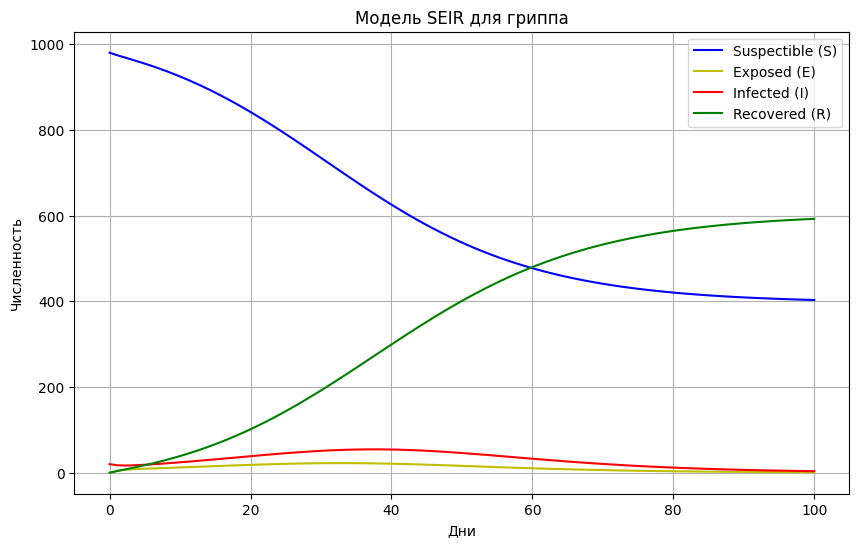
\includegraphics[scale=0.6]{images/graph01}
	 	\caption{График численного решения задачи Коши для детерминированной SEIR модели}
	 	\label{fig:graph01}
	 \end{figure}
	 
	 Из графика видно, как сперва число здоровых людей начинает стремительно уменьшатся, пока не достигает грани в 400. Число выздоровевших же напротив начинает стремительно возрастать, пересекается с график числа здоровых людей на 60-ый день, а затем скорость становится все ниже и ниже, пока не достигается грань в 600 человек. Как можно видеть, через 100 дней после начала эпидемии число болеющих практически снизилось до нуля. То есть мы можем заключить, что приблизительно спустя 100 дней эпидемия прекратилась.
	\section{Применение вероятностной SEIR модели для моделирования}
	В соответствии с п.2.1.1 построим вероятностную модель с дискретным временем, поскольку для нее легко привести численную реализацию. Вероятностная SEIR-модель для гриппа имеет следующий вид
	\begin{equation}
		\begin{dcases}
			S_{t+1} = S_t - \Delta E_t,\\
			E_{t+1} = E_t +\Delta E_t - \Delta I_t,\\
			I_{t+1} = I_t + \Delta I_t - \Delta R_t,\\
			R_{t+1} = R_t + \Delta R_t,
			S_0 = 980,\ E_0 = 0,\ I_0 = 20,\ \ R_0 = 0
		\end{dcases}
		t = 0,1,2\ldots,
	\end{equation}
	при этом
	$$\Delta E_t \sim \Binom\left(S_t, 
	1 - \exp\left(-\beta\cdot  \frac{I}{N} \cdot \Delta t\right)\right),$$
	$$\Delta I_t \sim \Binom\left(E_t, 1 - \exp\left(-\sigma \cdot \Delta t\right)\right),$$
	$$\Delta R_t \sim \Binom\left(I_t, 1 - \exp\left(-\gamma \cdot \Delta t\right)\right).$$
	
	Таким образом, мы можем описать процесс распространения гриппа с помощью вероятностной SEIR модели. Приведем 100 реализаций этой модели, а в качестве результирующего графика выберем средние значения для каждой группы, а также приведем 95\%-доверительные интервалы для каждой переменной (Приложение 2)
	
	\begin{figure}[h]
		\centering
		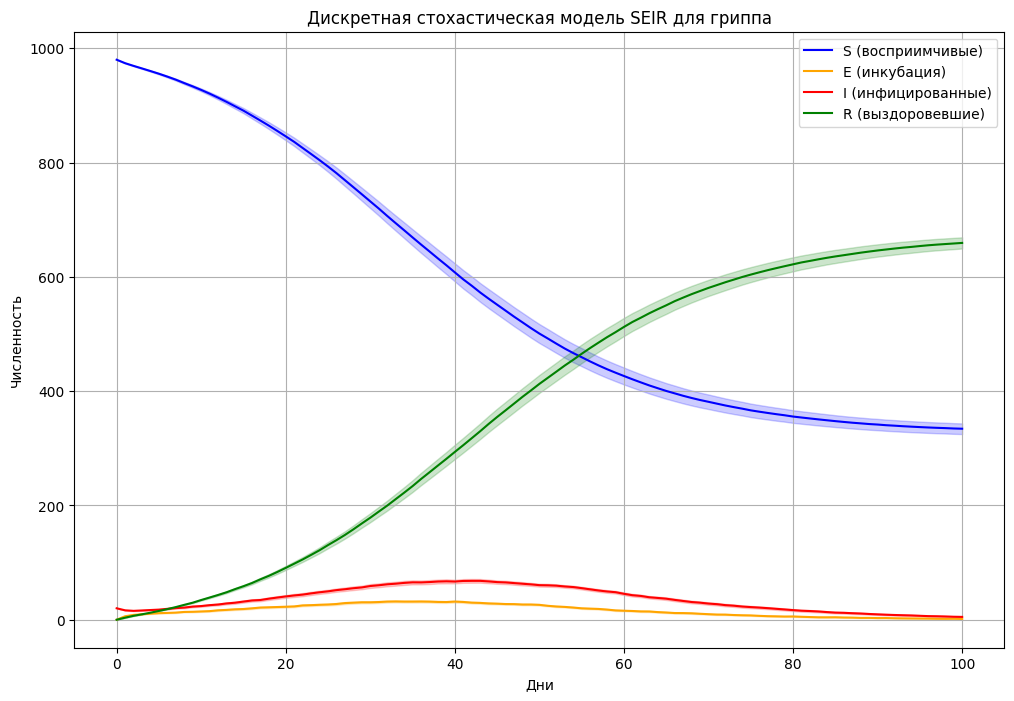
\includegraphics[scale=0.5]{images/graph02}
		\caption{График численной реализация вероятностной SEIR для гриппа с доверительными интервалами}
		\label{fig:graph02}
	\end{figure}
	
	Из графика видно, что поведения функций, описывающих группы людей, не сильно изменились относительно детерминированного случая. Однако теперь сместились границы, при которых число восприимчивых людей перестает снижаться, а число выздоровевших -- расти. 
	
	\section{Применение пространственной SEIR модели для моделирования}
	Для пространственной модели построим сетку узлов $30 \times 30$ на которой зададим вероятностную SEIR-модель для дискретного времени с сохранением всех параметров из предыдущего случая. Клетки, в которых будут находиться инфицированные люди, будут выбираться случайно.
	
	Таким образом, мы можем описать процесс распространения гриппа с помощью вероятностной SEIR-модели в пространстве. Приведем на графике одну из реализаций через каждые 10 дней (Приложение 3)
	
	\begin{figure}[h]
		\centering
		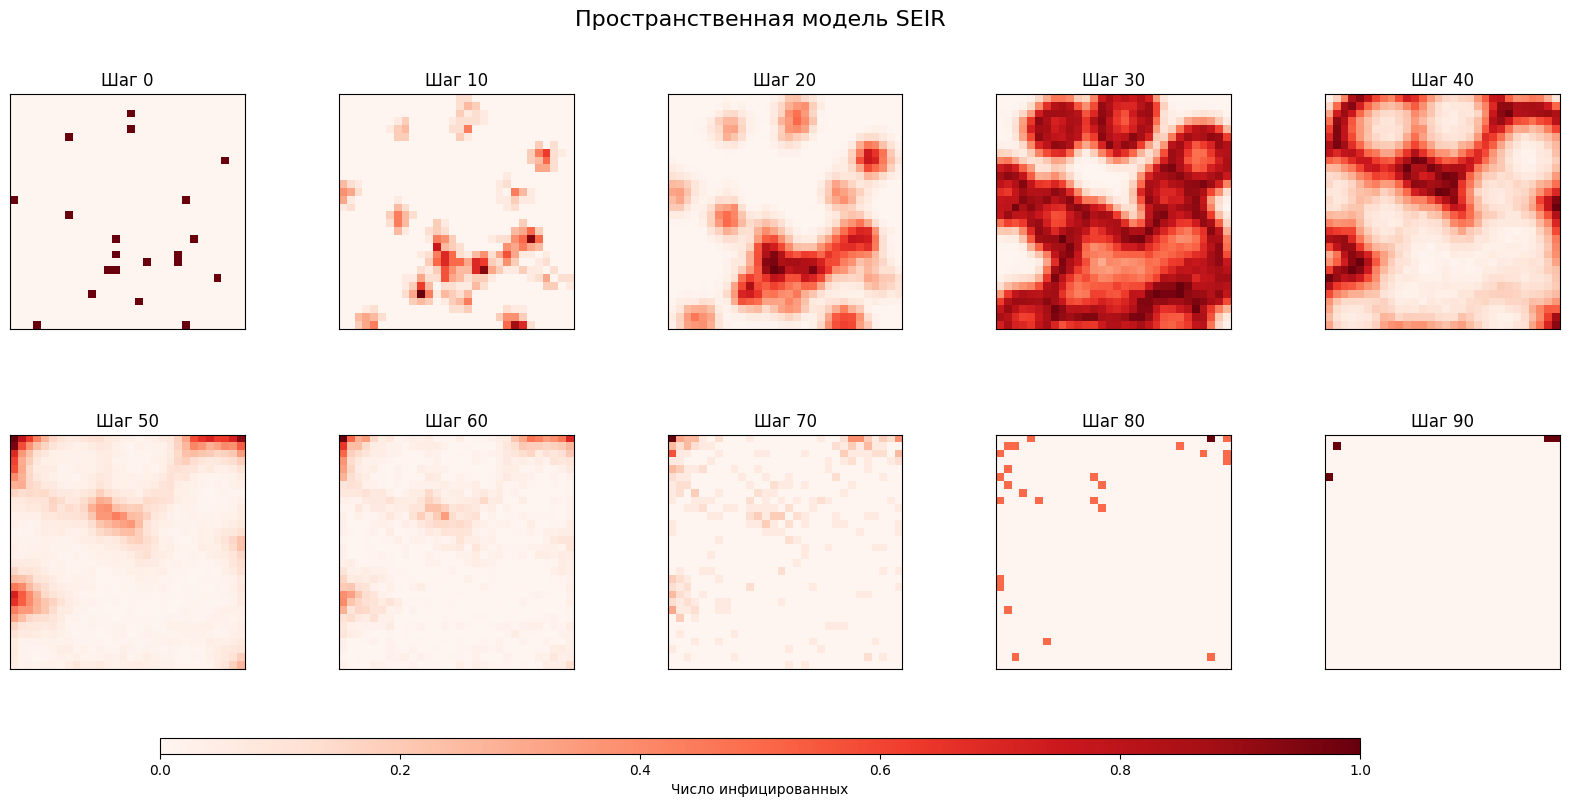
\includegraphics[scale=0.4]{images/graph03}
		\caption{Пространственные графики численной реализации вероятностной SEIR модели для гриппа}
		\label{fig:graph03}
	\end{figure}
	
	Из построенных графиков видно, что, как и в предыдущих случаях, спустя 30-40 дней число инфицированных особей достигает своего пика, а затем стремительно снижается до такой степени, что уже на 90-ый день число инфицированных стремится к нулю. Кроме этого также заметно, как все эти изменения отражаются в пространстве.
	
	\section{Применение мультиагентной SEIR модели для моделирования}
	Алгоритм моделирует распространение инфекции в популяции агентов, используя модифицированную модель SEIR (восприимчивые, экспонированные, инфицированные, выздоровевшие). Популяция агентов размещена в двумерном пространстве, и их поведение включает перемещение, заражение и смену состояния в зависимости от времени и контактов с другими агентами. Графики показывают динамику агентов на разных временных шагах.
	
	\subsubsection*{Шаг 1}
	
	На первом этапе создаётся популяция агентов с заданными свойствами:
	
	\begin{itemize}
		\item {Количество агентов ($N_{\text{agents}}$)}: Всего агентов в симуляции.
		\item {Позиции агентов}: Каждый агент случайным образом размещается в двумерном пространстве размера $L \times L$.
		\item {Индивидуальные параметры агентов}: Для каждого агента задаются случайные значения:
		\begin{itemize}
			\item {Восприимчивость ($\text{susceptibility}$)}: Коэффициент, влияющий на вероятность заражения.
			\item {Интенсивность контактов ($\text{contact\_rate}$)}: Сколько контактов совершает агент.
			\item {Инкубационный период ($\text{incubation\_period}$)}: Время, необходимое для перехода из состояния <<Экспонированный>> (E) в <<Инфицированный>> (I).
			\item {Инфекционный период ($\text{infectious\_period}$)}: Время, через которое инфицированный агент выздоравливает.
		\end{itemize}
		\item {Начальное состояние}: Большинство агентов находятся в состоянии <<Восприимчивые>> (S). Несколько агентов (определяется параметром\\ initial\_infected) изначально заражены (I).
	\end{itemize}
	
	\subsubsection*{Шаг 2}
	
	На каждом временном шаге ($T$) выполняются следующие действия для обновления состояния агентов:
	
	\begin{enumerate}
		\item Перемещение агентов
		\begin{itemize}
		\item Каждый агент с заданной вероятностью ($\text{move\_prob}$) перемещается случайным образом в пределах пространства.
		\item Если агент выходит за границы пространства, его позиция корректируется (ограничивается рамками пространства $L \times L$).
		\end{itemize}
		\item Обновление состояния агента
		\begin{itemize}
		\item {Если агент в состоянии <<Экспонированный>> (E)}:
		\begin{itemize}
			\item Увеличивается таймер заражения ($\text{time\_infected}$).
			\item Если время заражения превышает инкубационный период, агент переходит в состояние <<Инфицированный>> (I).
		\end{itemize}
		\item {Если агент в состоянии <<Инфицированный>> (I)}:
		\begin{itemize}
			\item Также увеличивается таймер заражения ($\text{time\_infected}$).
			\item Если таймер превышает инфекционный период, агент переходит в состояние <<Выздоровевший>> (R).
		\end{itemize}
		\end{itemize}
		\item Заражение других агентов
		\begin{itemize}
		\item Если агент находится в состоянии <<Инфицированный>> (I), он может заразить других агентов, находящихся рядом (расстояние меньше 0.5).
		\item Вероятность заражения определяется формулой:
		\[
		P_{\text{infect}} = \beta \cdot \text{susceptibility},
		\]
		где $\beta$~--- коэффициент передачи инфекции.
		\item Если случайное число меньше $P_{\text{infect}}$, агент в состоянии <<Восприимчивый>> (S) переходит в состояние <<Экспонированный>> (E), и его таймер заражения сбрасывается.
		\end{itemize}
	\end{enumerate}
	
	\subsubsection*{Шаг 3}
	
	Каждые 10 временных шагов (или другой заданный интервал) сохраняется:
	\begin{itemize}
		\item Текущее состояние всех агентов.
		\item Время ($t$), соответствующее этому состоянию.
	\end{itemize}
	
	Эти данные используются для построения графиков.
	
	\subsubsection*{Шаг 4}
	
	Создаётся сетка из графиков, отображающих положение агентов в пространстве на разных временных шагах. Каждый график отражает состояние популяции в конкретный момент времени.
	
	{Цветовое кодирование состояния агентов}:
		\begin{itemize}
			\item {Синий (S)}~--- восприимчивые агенты.
			\item {Оранжевый (E)}~--- экспонированные агенты.
			\item {Красный (I)}~--- инфицированные агенты.
			\item {Зелёный (R)}~--- выздоровевшие агенты.
		\end{itemize}
	
	\subsubsection*{Используемые параметры и их влияние}
	
	\begin{itemize}
		\item {$N_{\text{agents}}$}~--- количество агентов:
		\begin{itemize}
			\item Чем больше агентов, тем плотнее популяция, что может ускорить распространение инфекции.
		\end{itemize}
		\item \textbf{$L$}~--- размер пространства:
		\begin{itemize}
			\item Чем больше пространство, тем сложнее агентам контактировать, что замедляет заражение.
		\end{itemize}
		\item \textbf{$\beta$}~--- коэффициент передачи:
		\begin{itemize}
			\item Определяет вероятность заражения при контакте. Чем выше, тем быстрее распространяется инфекция.
		\end{itemize}
		\item {$\sigma_{\text{mean}}$ и $\gamma_{\text{mean}}$}~--- инкубационный и инфекционный периоды:
		\begin{itemize}
			\item Увеличение этих параметров замедляет переход между состояниями, что влияет на динамику эпидемии.
		\end{itemize}
		\item {$\text{move\_prob}$}~--- вероятность перемещения агентов:
		\begin{itemize}
			\item Чем больше значение, тем чаще агенты перемещаются, что увеличивает вероятность контактов и заражения.
		\end{itemize}
		\item {$\text{initial\_infected}$}~--- начальное число заражённых:
		\begin{itemize}
			\item Определяет начальный уровень инфекции. Чем больше заражённых в начале, тем быстрее эпидемия распространяется.
		\end{itemize}
	\end{itemize}
	
	Приведем графический результат работы алгоритма
	
	\begin{figure}[h]
		\centering
		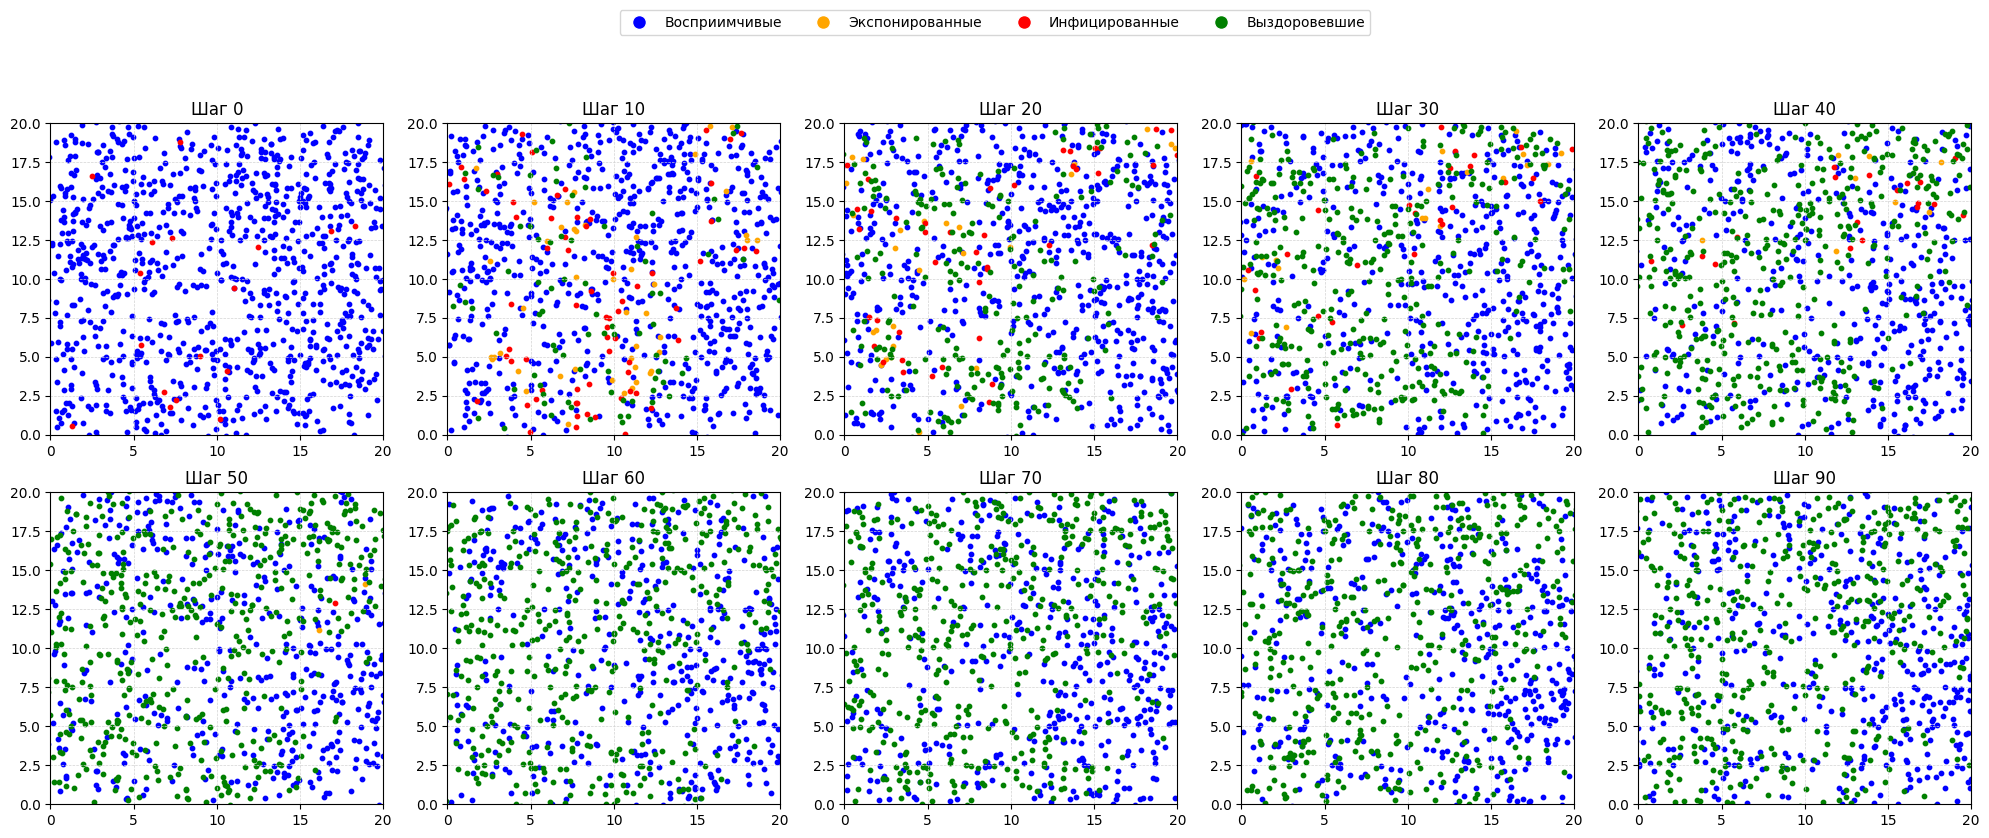
\includegraphics[scale=0.3]{images/graph04}
		\caption{Графическое представление реализации мультиагентной SEIR модели}
		\label{fig:graph04}
	\end{figure}
	
	Таким образом, можно заметить, что теперь процесс распространения гриппа протекает иначе. Основной пике был между 10-ым и 20-ым днями, а далее после 60-го дня грипп не распространялся, то есть распространение прекратилось. Можно сделать выводы, что наличие у каждого индивида особых собственных свойств сильно сказывается на процессе распространения заболевания.
	
	
	\chapter*{ЗАКЛЮЧЕНИЕ}\addcontentsline{toc}{section}{ЗАКЛЮЧЕНИЕ}
	В данной работе рассмотрена SEIR-модель и ее расширения, с помощью которых был смоделирован процесс распространения заболеваний.
	В ходе работы
	\begin{enumerate}
		\item рассмотрена классическая SI-модель и ее аналитическое решение;
		\item рассмотрена классическая SIR-модель, вывод ее дифференциальных уравнений, исследование вопроса о корректной постановке задачи Коши, построение аналитического решения, описание методов построения приближенного решения;
		\item рассмотрены основные базовые модификации SIR-модели: SIS, SIRS, SIRD, SEIR, MSIR, MSEIR;
		\item рассмотрены расширения базовой SEIR модели: вероятностная модель, пространственная модель, мультиагентная модель;
		\item на практике были рассмотрены способы построения расширений для модели SEIR для решения задачи о моделировании распространения гриппа и приведены результаты моделирования.
	\end{enumerate}
	
	\newpage
	\chapter*{СПИСОК ИСТОЧНИКОВ}\addcontentsline{toc}{section}{СПИСОК ИСТОЧНИКОВ}
	\begin{enumerate}
		\item Statistical forecasting of the dynamics of epidemiological indicators for COVID-19 incidence in the Republic of Belarus / Yu. S. Kharin, V. A. Valoshka, O. V. Dernakova, V. I. Malugin, A. Yu. Kharin// Journal of the Belarusian State University. Mathematics and Informatics. - 2020. - № 3. - С. 36-50
		\item Methods of intellectual data analysis in COVID-19 research / O. V. Senko, A. V. Kuznetsova, E. M. Voronin, O. A. Kravtsova, L. R. Borisova, I. L. Kirilyuk, V. G. Akimkin// Journal of the Belarusian State University. Mathematics and Informatics. – 2022. – № 1. – С. 83-96
		\item Детерминированные и стохастические модели распространения инфекции и тестирование в изолированном контингенте/ Чигарев, А. В., Журавков, М. А., Чигарев, В. А.// Журнал Белорусского государственного университета. Математика. Информатика - 2021. - № 3. - С. 57-67
		\item Lazzizzera, I. (2021) An Analytic Approximate Solution of the SIR Model. Applied Mathematics, 12, 58-73
		\item Contribution to the Mathematical Theory of Epidemics. Proceedings of the Royal Socoety A/ Kermack, W.O. and McKendrick, A.G. (1927) //115, 700-721.
		\item МАТЕМАТИЧЕСКАЯ ЭПИДЕМИОЛОГИЯ Учебно–методическое пособие
		по выполнению лабораторных работ / В. Н. Леоненко // УНИВЕРСИТЕТ ИТМО Санкт–Петербург. -- 2018. С. 10-30
		\item Грипп -- Википедия: [Электронный ресурс]. URL:\\ https://ru.wikipedia.org/wiki/Грипп. (Дата обращения 17.12.2024).
		\item Индекс репродукции -- Википедия: [Электронный ресурс]. URL:\\
		https://ru.wikipedia.org/wiki/Индекс\_репродукции. 
		(Дата обращения\\ 17.12.2024)
	\end{enumerate}
	\newpage
	\chapter*{ПРИЛОЖЕНИЕ}\addcontentsline{toc}{section}{ПРИЛОЖЕНИЕ}
	\section*{Приложение 1}\addcontentsline{toc}{subsection}{Приложение 1}
	\begin{verbatim}
import numpy as np
from scipy.integrate import odeint
import matplotlib.pyplot as plt

# Параметры модели
N = 1000  # Общее население
sigma = 1/2  # 1 / Инкубационный период
gamma = 1/5  # 1 / Инфекционный период
R0 = 1.5  # Базовое репродуктивное число
beta = R0 * gamma  # Расчет beta

# Начальное число инфицированных и восприимчивых
I0 = 20
E0 = 0
R0 = 0
S0 = N - I0 - E0 - R0

# Время моделирования (в днях)
t = np.linspace(0, 100, 100)  # 100 дней

# Модель SEIR
def seir_model(y, t, N, beta, sigma, gamma):
S, E, I, R = y
dSdt = -beta * S * I / N
dEdt = beta * S * I / N - sigma * E
dIdt = sigma * E - gamma * I
dRdt = gamma * I
return dSdt, dEdt, dIdt, dRdt

# Начальные условия
y0 = S0, E0, I0, R0

# Решение дифференциальных уравнений
result = odeint(seir_model, y0, t, args=(N, beta, sigma, gamma))
S, E, I, R = result.T

# Построение графиков
plt.figure(figsize=(10, 6))
plt.plot(t, S, 'b', label='Suspectible (S)')
plt.plot(t, E, 'y', label='Exposed (E)')
plt.plot(t, I, 'r', label='Infected (I)')
plt.plot(t, R, 'g', label='Recovered (R)')
plt.xlabel('Дни')
plt.ylabel('Численность')
plt.legend()
plt.title('Модель SEIR для гриппа')
plt.grid()
plt.show()
	\end{verbatim}
	\section*{Приложение 2}\addcontentsline{toc}{subsection}{Приложение 2}
\begin{verbatim}
import numpy as np
import matplotlib.pyplot as plt

def stochastic_seir_discrete(N, beta, sigma, gamma, 
		S0, E0, I0, R0, days, runs):
results = []
for _ in range(runs):
# Инициализация
S, E, I, R = S0, E0, I0, R0
S_history, E_history, I_history, R_history = [S], [E], [I], [R]

for t in range(days):
# Вычисление вероятностей
P_infect = 1 - np.exp(-beta * I / N)
P_incub = 1 - np.exp(-sigma)
P_recover = 1 - np.exp(-gamma)

# Случайные переходы
new_infected = np.random.binomial(S, P_infect)
new_exposed = np.random.binomial(E, P_incub)
new_recovered = np.random.binomial(I, P_recover)

# Обновление численностей
S -= new_infected
E += new_infected - new_exposed
I += new_exposed - new_recovered
R += new_recovered

# Сохранение истории
S_history.append(S)
E_history.append(E)
I_history.append(I)
R_history.append(R)

results.append((S_history, E_history, I_history, R_history))

return results

# Параметры
N = 1000
sigma = 1 / 2
gamma = 1 / 5
R_0 = 1.5
beta = R_0 * gamma
E0 = 0
I0 = 20
R0 = 0
S0 = N - E0 - I0 - R0
days = 100
runs = 100

# Запуск модели
results = stochastic_seir_discrete(N, beta, sigma, gamma, 
		S0, E0, I0, R0, days, runs)

# Построение средних значений и стандартных отклонений
S_all = np.array([res[0] for res in results])
E_all = np.array([res[1] for res in results])
I_all = np.array([res[2] for res in results])
R_all = np.array([res[3] for res in results])

S_avg = np.mean(S_all, axis=0)
E_avg = np.mean(E_all, axis=0)
I_avg = np.mean(I_all, axis=0)
R_avg = np.mean(R_all, axis=0)

S_std = np.std(S_all, axis=0)
E_std = np.std(E_all, axis=0)
I_std = np.std(I_all, axis=0)
R_std = np.std(R_all, axis=0)

# Квантиль нормального распределения для 95% доверительного интервала
z = 1.96

# Вычисление доверительных интервалов
S_CI_lower = S_avg - z * S_std / np.sqrt(runs)
S_CI_upper = S_avg + z * S_std / np.sqrt(runs)

E_CI_lower = E_avg - z * E_std / np.sqrt(runs)
E_CI_upper = E_avg + z * E_std / np.sqrt(runs)

I_CI_lower = I_avg - z * I_std / np.sqrt(runs)
I_CI_upper = I_avg + z * I_std / np.sqrt(runs)

R_CI_lower = R_avg - z * R_std / np.sqrt(runs)
R_CI_upper = R_avg + z * R_std / np.sqrt(runs)

# График
plt.figure(figsize=(12, 8))

# Восприимчивые (S)
plt.plot(S_avg, label='S (восприимчивые)', color='blue')
plt.fill_between(range(days + 1), S_CI_lower, S_CI_upper, 
		color='blue', alpha=0.2)

# Экспонированные (E)
plt.plot(E_avg, label='E (инкубация)', color='orange')
plt.fill_between(range(days + 1), E_CI_lower, E_CI_upper, 
		color='orange', alpha=0.2)

# Инфицированные (I)
plt.plot(I_avg, label='I (инфицированные)', color='red')
plt.fill_between(range(days + 1), I_CI_lower, I_CI_upper, 
		color='red', alpha=0.2)

# Выздоровевшие (R)
plt.plot(R_avg, label='R (выздоровевшие)', color='green')
plt.fill_between(range(days + 1), R_CI_lower, R_CI_upper, 
		color='green', alpha=0.2)

# Оформление
plt.xlabel('Дни')
plt.ylabel('Численность')
plt.title('Дискретная стохастическая модель SEIR для гриппа')
plt.legend()
plt.grid()
plt.show()
\end{verbatim}
\subsection*{Приложение 3}
\begin{verbatim}
import numpy as np
import matplotlib.pyplot as plt

# Параметры модели
M, N = 30, 30  # Размерность решетки
sigma = 1 / 2  # Инкубационный период
gamma = 1 / 5   # Инфекционный период
R_0 = 1.5 # Базовое репродуктивное число 
beta = R_0 * gamma   # Коэффициент передачи
T = 100          # Число временных шагов
initial_infected = 20  # Начальное количество зараженных

# Создание сетки
def initialize_grid(M, N, initial_infected):
grid = np.zeros((M, N, 4))  # [S, E, I, R] для каждой ячейки
grid[:, :, 0] = 1000  # Изначально все восприимчивы (S = 1000)

# Случайно заражаем несколько ячеек
for _ in range(initial_infected):
x, y = np.random.randint(0, M), np.random.randint(0, N)
grid[x, y, 0] -= 1  # Уменьшаем восприимчивых
grid[x, y, 2] += 1  # Добавляем инфицированных (I)

return grid

# Обновление состояния ячеек
def update_grid(grid, beta, sigma, gamma, M, N):
new_grid = grid.copy()
for i in range(M):
for j in range(N):
S, E, I, R = grid[i, j]

# Считаем влияние соседей
neighbors = [(i-1, j), (i+1, j), (i, j-1), (i, j+1)]
total_infected = I
for ni, nj in neighbors:
if 0 <= ni < M and 0 <= nj < N:
total_infected += grid[ni, nj, 2]

# Вероятность заражения
P_infect = 1 - np.exp(-beta * total_infected / 1000)

# Переходы между состояниями
new_infected = np.random.binomial(S, P_infect)
new_exposed = np.random.binomial(E, sigma)
new_recovered = np.random.binomial(I, gamma)

# Обновление численностей
new_grid[i, j, 0] -= new_infected  # S уменьшается
new_grid[i, j, 1] += new_infected - new_exposed  # E
new_grid[i, j, 2] += new_exposed - new_recovered  # I
new_grid[i, j, 3] += new_recovered  # R

return new_grid

# Визуализация сетки
def plot_grid_in_subplot(ax, grid, t):
I_grid = grid[:, :, 2]  # Берем слой с инфицированными (I)
im = ax.imshow(I_grid, cmap='Reds', interpolation='nearest')
ax.set_title(f'Шаг {t}')
ax.set_xticks([])
ax.set_yticks([])
return im

# Запуск модели
grid = initialize_grid(M, N, initial_infected)

# Создание сетки для графиков
fig, axes = plt.subplots(2, 5, figsize=(20, 8)) 
axes = axes.flatten()  # Упрощаем доступ к подграфикам

for idx, t in enumerate(range(T)):
# Построение графика в соответствующем подграфике
if t % 10 == 0: 
plot_grid_in_subplot(axes[int(idx/10)], grid, t)
grid = update_grid(grid, beta, sigma, gamma, M, N)

# Общий заголовок
fig.suptitle('Пространственная модель SEIR', fontsize=16)

# Увеличиваем отступы между графиками и цветовой шкалой
plt.subplots_adjust(bottom=0.15, top=0.88, wspace=0.4, hspace=0.4)

# Создаем отдельную область для colorbar
cbar_ax = fig.add_axes([0.2, 0.05, 0.6, 0.02])
cbar = fig.colorbar(
plt.cm.ScalarMappable(cmap='Reds'),
cax=cbar_ax,
orientation='horizontal'
)
cbar.set_label('Число инфицированных')

# Оформление и вывод
plt.show()
\end{verbatim}
\subsection*{Приложение 4}
\begin{verbatim}
import numpy as np
import matplotlib.pyplot as plt

# Параметры модели
N_agents = 1000      # Число агентов
L = 20               # Размер пространства (L x L)
beta = 0.3           # Базовый коэффициент передачи
sigma_mean = 2       # Средний инкубационный период
gamma_mean = 5       # Средний инфекционный период
T = 100              # Число временных шагов
initial_infected = 20  # Начальное количество зараженных
move_prob = 0.8      # Вероятность перемещения агента

# Инициализация агентов
def initialize_agents(N_agents, L, initial_infected):
agents = []
for i in range(N_agents):
agent = {
	"state": "S", 
	"position": np.random.rand(2) * L,  
	"susceptibility": np.random.uniform(0.8, 1.2), 
	"contact_rate": np.random.uniform(0.5, 1.5), 
	"incubation_period": np.random.poisson(sigma_mean), 
	"infectious_period": np.random.poisson(gamma_mean), 
	"time_infected": 0  # Время с момента заражения
}
agents.append(agent)

# Заражаем нескольких агентов
for i in range(initial_infected):
agents[i]["state"] = "I"

return agents

# Обновление состояния агентов
def update_agents(agents, L, beta, move_prob):
for agent in agents:
# Перемещение агента
if np.random.rand() < move_prob:
agent["position"] += np.random.uniform(-1, 1, 2)
agent["position"] = np.clip(agent["position"], 0, L)

# Обновление состояний
if agent["state"] == "E":
agent["time_infected"] += 1
if agent["time_infected"] >= agent["incubation_period"]:
agent["state"] = "I"  # Переход в инфекционное состояние

elif agent["state"] == "I":
agent["time_infected"] += 1
if agent["time_infected"] >= agent["infectious_period"]:
agent["state"] = "R"  # Выздоровление

# Проверка контактов и заражение
for i, agent in enumerate(agents):
if agent["state"] == "I":
for j, other_agent in enumerate(agents):
if i != j and other_agent["state"] == "S":
# Рассчитываем расстояние между агентами
dist = np.linalg.norm(agent["position"] - other_agent["position"])
if dist < 0.5:  # Если агенты близко друг к другу
P_infect = beta * other_agent["susceptibility"]
if np.random.rand() < P_infect:
other_agent["state"] = "E"  # Агент становится экспонированным
other_agent["time_infected"] = 0  # Сбрасываем таймер

# Визуализация графиков с общей легендой
def plot_agents_grid(agents_list, time_points, L):
colors = {"S": "blue", "E": "orange", "I": "red", "R": "green"}
labels = {"S": "Восприимчивые", "E": "Экспонированные", 
	"I": "Инфицированные", "R": "Выздоровевшие"}

fig, axes = plt.subplots(2, 5, figsize=(20, 8))
axes = axes.flatten()

for idx, (agents, t) in enumerate(zip(agents_list, time_points)):
ax = axes[idx]
for state, color in colors.items():
state_agents = [agent for agent in agents if agent["state"] == state]
positions = np.array([agent["position"] for agent in state_agents])
if len(positions) > 0:
ax.scatter(positions[:, 0], positions[:, 1], color=color, 
	label=labels[state], s=10)

ax.set_title(f"Шаг {t}")
ax.set_xlim(0, L)
ax.set_ylim(0, L)
ax.grid(color="lightgray", linestyle="--", linewidth=0.5)

# Добавление общей легенды
handles = [plt.Line2D([0], [0], marker='o', color='w', 
	markerfacecolor=color, markersize=10, label=label) 
for label, color in zip(labels.values(), colors.values())]
fig.legend(handles=handles, loc='upper center', ncol=4, 
	bbox_to_anchor=(0.5, 1.05))

plt.tight_layout()
plt.subplots_adjust(top=0.9) 
plt.show()

# Запуск модели
agents = initialize_agents(N_agents, L, initial_infected)

# Список для хранения агентов на выбранных шагах
agents_list = []
time_points = []

for t in range(T):
if t % 10 == 0:  # Сохраняем состояние каждые 10 шагов
agents_list.append([agent.copy() for agent in agents])  
time_points.append(t)
update_agents(agents, L, beta, move_prob)

# Отображаем 10 графиков
plot_agents_grid(agents_list[:10], time_points[:10], L)
\end{verbatim}
\end{document}